\documentclass[a4paper]{book}
\usepackage{makeidx}
\usepackage{natbib}
\usepackage{graphicx}
\usepackage{multicol}
\usepackage{float}
\usepackage{listings}
\usepackage{color}
\usepackage{ifthen}
\usepackage[table]{xcolor}
\usepackage{textcomp}
\usepackage{alltt}
\usepackage{ifpdf}
\ifpdf
\usepackage[pdftex,
            pagebackref=true,
            colorlinks=true,
            linkcolor=blue,
            unicode
           ]{hyperref}
\else
\usepackage[ps2pdf,
            pagebackref=true,
            colorlinks=true,
            linkcolor=blue,
            unicode
           ]{hyperref}
\usepackage{pspicture}
\fi
\usepackage[utf8]{inputenc}
\usepackage{mathptmx}
\usepackage[scaled=.90]{helvet}
\usepackage{courier}
\usepackage{sectsty}
\usepackage[titles]{tocloft}
\usepackage{doxygen}
\lstset{language=C++,inputencoding=utf8,basicstyle=\footnotesize,breaklines=true,breakatwhitespace=true,tabsize=8,numbers=left }
\makeindex
\setcounter{tocdepth}{3}
\renewcommand{\footrulewidth}{0.4pt}
\renewcommand{\familydefault}{\sfdefault}
\hfuzz=15pt
\setlength{\emergencystretch}{15pt}
\hbadness=750
\tolerance=750
\begin{document}
\hypersetup{pageanchor=false,citecolor=blue}
\begin{titlepage}
\vspace*{7cm}
\begin{center}
{\Large \-Py\-R\-T\-A\-I }\\
\vspace*{1cm}
{\large \-Generated by Doxygen 1.7.5}\\
\vspace*{0.5cm}
{\small Wed May 9 2012 10:32:22}\\
\end{center}
\end{titlepage}
\clearemptydoublepage
\pagenumbering{roman}
\tableofcontents
\clearemptydoublepage
\pagenumbering{arabic}
\hypersetup{pageanchor=true,citecolor=blue}
\chapter{\-Namespace \-Index}
\section{\-Packages}
\-Here are the packages with brief descriptions (if available)\-:\begin{DoxyCompactList}
\item\contentsline{section}{\hyperlink{namespacecustom__exceptions}{custom\-\_\-exceptions} \\*\-Custom exceptions for the library }{\pageref{namespacecustom__exceptions}}{}
\item\contentsline{section}{\hyperlink{namespacepyrtai}{pyrtai} \\*\-This package handles the configurations }{\pageref{namespacepyrtai}}{}
\item\contentsline{section}{\hyperlink{namespacepyrtai_1_1configurator}{pyrtai\-::configurator} }{\pageref{namespacepyrtai_1_1configurator}}{}
\item\contentsline{section}{\hyperlink{namespacepyrtai_1_1connector}{pyrtai\-::connector} }{\pageref{namespacepyrtai_1_1connector}}{}
\item\contentsline{section}{\hyperlink{namespacepyrtai_1_1custom__exceptions}{pyrtai\-::custom\-\_\-exceptions} }{\pageref{namespacepyrtai_1_1custom__exceptions}}{}
\item\contentsline{section}{\hyperlink{namespacepyrtai_1_1data__collector}{pyrtai\-::data\-\_\-collector} }{\pageref{namespacepyrtai_1_1data__collector}}{}
\item\contentsline{section}{\hyperlink{namespacepyrtai_1_1data__poller}{pyrtai\-::data\-\_\-poller} }{\pageref{namespacepyrtai_1_1data__poller}}{}
\item\contentsline{section}{\hyperlink{namespacepyrtai_1_1rtai__server}{pyrtai\-::rtai\-\_\-server} }{\pageref{namespacepyrtai_1_1rtai__server}}{}
\item\contentsline{section}{\hyperlink{namespacepyrtai_1_1target}{pyrtai\-::target} }{\pageref{namespacepyrtai_1_1target}}{}
\item\contentsline{section}{\hyperlink{namespacepyrtai_1_1utility}{pyrtai\-::utility} }{\pageref{namespacepyrtai_1_1utility}}{}
\end{DoxyCompactList}

\chapter{\-Class \-Index}
\section{\-Class \-Hierarchy}
\-This inheritance list is sorted roughly, but not completely, alphabetically\-:\begin{DoxyCompactList}
\item \contentsline{section}{pyrtai\-:\-:configurator\-:\-:\-Configurator}{\pageref{classpyrtai_1_1configurator_1_1_configurator}}{}
\item \contentsline{section}{pyrtai\-:\-:connector\-:\-:\-Connector}{\pageref{classpyrtai_1_1connector_1_1_connector}}{}
\item \contentsline{section}{pyrtai\-:\-:data\-\_\-collector\-:\-:\-Data\-Collector}{\pageref{classpyrtai_1_1data__collector_1_1_data_collector}}{}
\item \contentsline{section}{pyrtai\-:\-:data\-\_\-poller\-:\-:\-Data\-Poller}{\pageref{classpyrtai_1_1data__poller_1_1_data_poller}}{}
\item \contentsline{section}{pyrtai\-:\-:custom\-\_\-exceptions\-:\-:\-Rtai\-Error}{\pageref{classpyrtai_1_1custom__exceptions_1_1_rtai_error}}{}
\begin{DoxyCompactList}
\item \contentsline{section}{pyrtai\-:\-:custom\-\_\-exceptions\-:\-:\-Rtai\-Config\-Error}{\pageref{classpyrtai_1_1custom__exceptions_1_1_rtai_config_error}}{}
\item \contentsline{section}{pyrtai\-:\-:custom\-\_\-exceptions\-:\-:\-Rtai\-Xml\-Rpc\-Error}{\pageref{classpyrtai_1_1custom__exceptions_1_1_rtai_xml_rpc_error}}{}
\end{DoxyCompactList}
\item \contentsline{section}{pyrtai\-:\-:rtai\-\_\-server\-:\-:\-Rtai\-Server}{\pageref{classpyrtai_1_1rtai__server_1_1_rtai_server}}{}
\item \contentsline{section}{pyrtai\-:\-:target\-:\-:\-Target}{\pageref{classpyrtai_1_1target_1_1_target}}{}
\end{DoxyCompactList}

\chapter{\-Class \-Index}
\section{\-Class \-List}
\-Here are the classes, structs, unions and interfaces with brief descriptions\-:\begin{DoxyCompactList}
\item\contentsline{section}{\hyperlink{classpyrtai_1_1configurator_1_1_configurator}{pyrtai\-::configurator\-::\-Configurator} \\*\hyperlink{classpyrtai_1_1configurator_1_1_configurator}{\-Configurator} class handles config values }{\pageref{classpyrtai_1_1configurator_1_1_configurator}}{}
\item\contentsline{section}{\hyperlink{classpyrtai_1_1connector_1_1_connector}{pyrtai\-::connector\-::\-Connector} \\*\-Connect to the \-R\-T\-A\-I server and manage responses and basic operations on it }{\pageref{classpyrtai_1_1connector_1_1_connector}}{}
\item\contentsline{section}{\hyperlink{classpyrtai_1_1data__collector_1_1_data_collector}{pyrtai\-::data\-\_\-collector\-::\-Data\-Collector} }{\pageref{classpyrtai_1_1data__collector_1_1_data_collector}}{}
\item\contentsline{section}{\hyperlink{classpyrtai_1_1data__poller_1_1_data_poller}{pyrtai\-::data\-\_\-poller\-::\-Data\-Poller} }{\pageref{classpyrtai_1_1data__poller_1_1_data_poller}}{}
\item\contentsline{section}{\hyperlink{classpyrtai_1_1custom__exceptions_1_1_rtai_config_error}{pyrtai\-::custom\-\_\-exceptions\-::\-Rtai\-Config\-Error} \\*\-Exception raised for errors involving connections }{\pageref{classpyrtai_1_1custom__exceptions_1_1_rtai_config_error}}{}
\item\contentsline{section}{\hyperlink{classpyrtai_1_1custom__exceptions_1_1_rtai_error}{pyrtai\-::custom\-\_\-exceptions\-::\-Rtai\-Error} \\*\-Base class for exceptions in this module }{\pageref{classpyrtai_1_1custom__exceptions_1_1_rtai_error}}{}
\item\contentsline{section}{\hyperlink{classpyrtai_1_1rtai__server_1_1_rtai_server}{pyrtai\-::rtai\-\_\-server\-::\-Rtai\-Server} }{\pageref{classpyrtai_1_1rtai__server_1_1_rtai_server}}{}
\item\contentsline{section}{\hyperlink{classpyrtai_1_1custom__exceptions_1_1_rtai_xml_rpc_error}{pyrtai\-::custom\-\_\-exceptions\-::\-Rtai\-Xml\-Rpc\-Error} \\*\-Exception raised for errors involving connections }{\pageref{classpyrtai_1_1custom__exceptions_1_1_rtai_xml_rpc_error}}{}
\item\contentsline{section}{\hyperlink{classpyrtai_1_1target_1_1_target}{pyrtai\-::target\-::\-Target} }{\pageref{classpyrtai_1_1target_1_1_target}}{}
\end{DoxyCompactList}

\chapter{\-File \-Index}
\section{\-File \-List}
\-Here is a list of all files with brief descriptions\-:\begin{DoxyCompactList}
\item\contentsline{section}{/home/drwolf/\-Devel/py\-R\-T\-A\-I/pyrtai/\hyperlink{____init_____8py}{\-\_\-\-\_\-init\-\_\-\-\_\-.\-py} }{\pageref{____init_____8py}}{}
\item\contentsline{section}{/home/drwolf/\-Devel/py\-R\-T\-A\-I/pyrtai/\hyperlink{configurator_8py}{configurator.\-py} }{\pageref{configurator_8py}}{}
\item\contentsline{section}{/home/drwolf/\-Devel/py\-R\-T\-A\-I/pyrtai/\hyperlink{connector_8py}{connector.\-py} }{\pageref{connector_8py}}{}
\item\contentsline{section}{/home/drwolf/\-Devel/py\-R\-T\-A\-I/pyrtai/\hyperlink{custom__exceptions_8py}{custom\-\_\-exceptions.\-py} }{\pageref{custom__exceptions_8py}}{}
\item\contentsline{section}{/home/drwolf/\-Devel/py\-R\-T\-A\-I/pyrtai/\hyperlink{data__collector_8py}{data\-\_\-collector.\-py} }{\pageref{data__collector_8py}}{}
\item\contentsline{section}{/home/drwolf/\-Devel/py\-R\-T\-A\-I/pyrtai/\hyperlink{data__poller_8py}{data\-\_\-poller.\-py} }{\pageref{data__poller_8py}}{}
\item\contentsline{section}{/home/drwolf/\-Devel/py\-R\-T\-A\-I/pyrtai/\hyperlink{rtai__server_8py}{rtai\-\_\-server.\-py} }{\pageref{rtai__server_8py}}{}
\item\contentsline{section}{/home/drwolf/\-Devel/py\-R\-T\-A\-I/pyrtai/\hyperlink{target_8py}{target.\-py} }{\pageref{target_8py}}{}
\item\contentsline{section}{/home/drwolf/\-Devel/py\-R\-T\-A\-I/pyrtai/\hyperlink{utility_8py}{utility.\-py} }{\pageref{utility_8py}}{}
\end{DoxyCompactList}

\chapter{\-Namespace \-Documentation}
\hypertarget{namespacecustom__exceptions}{
\section{custom\-\_\-exceptions \-Namespace \-Reference}
\label{namespacecustom__exceptions}\index{custom\-\_\-exceptions@{custom\-\_\-exceptions}}
}


\-Custom exceptions for the library.  




\subsection{\-Detailed \-Description}
\-Custom exceptions for the library. 
\hypertarget{namespacepyrtai}{
\section{pyrtai \-Namespace \-Reference}
\label{namespacepyrtai}\index{pyrtai@{pyrtai}}
}


\-This package handles the configurations.  


\subsection*{\-Packages}
\begin{DoxyCompactItemize}
\item 
namespace \hyperlink{namespacepyrtai_1_1configurator}{configurator}
\item 
namespace \hyperlink{namespacepyrtai_1_1connector}{connector}
\item 
namespace \hyperlink{namespacepyrtai_1_1custom__exceptions}{custom\-\_\-exceptions}
\item 
namespace \hyperlink{namespacepyrtai_1_1data__collector}{data\-\_\-collector}
\item 
namespace \hyperlink{namespacepyrtai_1_1data__poller}{data\-\_\-poller}
\item 
namespace \hyperlink{namespacepyrtai_1_1rtai__server}{rtai\-\_\-server}
\item 
namespace \hyperlink{namespacepyrtai_1_1target}{target}
\item 
namespace \hyperlink{namespacepyrtai_1_1utility}{utility}
\end{DoxyCompactItemize}


\subsection{\-Detailed \-Description}
\-This package handles the configurations. \-Various useful functions.

\-Represents the target server (master or slave)

\-Handles the connection to the \-R\-T\-A\-I server.

\begin{DoxySeeAlso}{\-See also}
\hyperlink{classpyrtai_1_1connector_1_1_connector}{pyrtai\-::connector\-::\-Connector}

\hyperlink{classpyrtai_1_1rtai__server_1_1_rtai_server}{pyrtai\-::rtai\-\_\-server\-::\-Rtai\-Server}

\hyperlink{classpyrtai_1_1target_1_1_target}{pyrtai\-::target\-::\-Target} \-T\-O\-D\-O\-: \-Gestire lo stato del \hyperlink{namespacepyrtai_1_1target}{target} 
\end{DoxySeeAlso}

\hypertarget{namespacepyrtai_1_1configurator}{
\section{pyrtai\-:\-:configurator \-Namespace \-Reference}
\label{namespacepyrtai_1_1configurator}\index{pyrtai\-::configurator@{pyrtai\-::configurator}}
}
\subsection*{\-Classes}
\begin{DoxyCompactItemize}
\item 
class \hyperlink{classpyrtai_1_1configurator_1_1_configurator}{\-Configurator}
\begin{DoxyCompactList}\small\item\em \hyperlink{classpyrtai_1_1configurator_1_1_configurator}{\-Configurator} class handles config values. \end{DoxyCompactList}\end{DoxyCompactItemize}

\hypertarget{namespacepyrtai_1_1connector}{
\section{pyrtai\-:\-:connector \-Namespace \-Reference}
\label{namespacepyrtai_1_1connector}\index{pyrtai\-::connector@{pyrtai\-::connector}}
}
\subsection*{\-Classes}
\begin{DoxyCompactItemize}
\item 
class \hyperlink{classpyrtai_1_1connector_1_1_connector}{\-Connector}
\begin{DoxyCompactList}\small\item\em \-The \hyperlink{classpyrtai_1_1connector_1_1_connector}{\-Connector} class connect to the \-R\-T\-A\-I server and manage responses and basic operations on it. \end{DoxyCompactList}\end{DoxyCompactItemize}

\hypertarget{namespacepyrtai_1_1custom__exceptions}{
\section{pyrtai\-:\-:custom\-\_\-exceptions \-Namespace \-Reference}
\label{namespacepyrtai_1_1custom__exceptions}\index{pyrtai\-::custom\-\_\-exceptions@{pyrtai\-::custom\-\_\-exceptions}}
}
\subsection*{\-Classes}
\begin{DoxyCompactItemize}
\item 
class \hyperlink{classpyrtai_1_1custom__exceptions_1_1_rtai_error}{\-Rtai\-Error}
\begin{DoxyCompactList}\small\item\em \-Base class for exceptions in this module. \end{DoxyCompactList}\item 
class \hyperlink{classpyrtai_1_1custom__exceptions_1_1_rtai_config_error}{\-Rtai\-Config\-Error}
\begin{DoxyCompactList}\small\item\em \-Exception raised for errors involving connections. \end{DoxyCompactList}\item 
class \hyperlink{classpyrtai_1_1custom__exceptions_1_1_rtai_xml_rpc_error}{\-Rtai\-Xml\-Rpc\-Error}
\begin{DoxyCompactList}\small\item\em \-Exception raised for errors involving connections. \end{DoxyCompactList}\end{DoxyCompactItemize}

\hypertarget{namespacepyrtai_1_1data__collector}{
\section{pyrtai\-:\-:data\-\_\-collector \-Namespace \-Reference}
\label{namespacepyrtai_1_1data__collector}\index{pyrtai\-::data\-\_\-collector@{pyrtai\-::data\-\_\-collector}}
}
\subsection*{\-Classes}
\begin{DoxyCompactItemize}
\item 
class \hyperlink{classpyrtai_1_1data__collector_1_1_data_collector}{\-Data\-Collector}
\end{DoxyCompactItemize}

\hypertarget{namespacepyrtai_1_1data__poller}{
\section{pyrtai\-:\-:data\-\_\-poller \-Namespace \-Reference}
\label{namespacepyrtai_1_1data__poller}\index{pyrtai\-::data\-\_\-poller@{pyrtai\-::data\-\_\-poller}}
}
\subsection*{\-Classes}
\begin{DoxyCompactItemize}
\item 
class \hyperlink{classpyrtai_1_1data__poller_1_1_data_poller}{\-Data\-Poller}
\end{DoxyCompactItemize}

\hypertarget{namespacepyrtai_1_1rtai__server}{
\section{pyrtai\-:\-:rtai\-\_\-server \-Namespace \-Reference}
\label{namespacepyrtai_1_1rtai__server}\index{pyrtai\-::rtai\-\_\-server@{pyrtai\-::rtai\-\_\-server}}
}
\subsection*{\-Classes}
\begin{DoxyCompactItemize}
\item 
class \hyperlink{classpyrtai_1_1rtai__server_1_1_rtai_server}{\-Rtai\-Server}
\end{DoxyCompactItemize}

\hypertarget{namespacepyrtai_1_1target}{
\section{pyrtai\-:\-:target \-Namespace \-Reference}
\label{namespacepyrtai_1_1target}\index{pyrtai\-::target@{pyrtai\-::target}}
}
\subsection*{\-Classes}
\begin{DoxyCompactItemize}
\item 
class \hyperlink{classpyrtai_1_1target_1_1_target}{\-Target}
\end{DoxyCompactItemize}

\hypertarget{namespacepyrtai_1_1utility}{
\section{pyrtai\-:\-:utility \-Namespace \-Reference}
\label{namespacepyrtai_1_1utility}\index{pyrtai\-::utility@{pyrtai\-::utility}}
}
\subsection*{\-Functions}
\begin{DoxyCompactItemize}
\item 
def \hyperlink{namespacepyrtai_1_1utility_a58a6904c0a7c5890e90137abd905feac}{get\-State\-From\-Response}
\begin{DoxyCompactList}\small\item\em \-Parses an integer state value which, converted into binary value, represents 4 states. \end{DoxyCompactList}\item 
def \hyperlink{namespacepyrtai_1_1utility_a5bfae0e64bb4701f2bfc4a59838ebdfc}{linesplit}
\begin{DoxyCompactList}\small\item\em \-Implements readline() with sockets. \end{DoxyCompactList}\end{DoxyCompactItemize}


\subsection{\-Function \-Documentation}
\hypertarget{namespacepyrtai_1_1utility_a58a6904c0a7c5890e90137abd905feac}{
\index{pyrtai\-::utility@{pyrtai\-::utility}!get\-State\-From\-Response@{get\-State\-From\-Response}}
\index{get\-State\-From\-Response@{get\-State\-From\-Response}!pyrtai::utility@{pyrtai\-::utility}}
\subsubsection[{get\-State\-From\-Response}]{\setlength{\rightskip}{0pt plus 5cm}def pyrtai\-::utility\-::get\-State\-From\-Response (
\begin{DoxyParamCaption}
\item[{}]{int\-\_\-state}
\end{DoxyParamCaption}
)}}
\label{namespacepyrtai_1_1utility_a58a6904c0a7c5890e90137abd905feac}


\-Parses an integer state value which, converted into binary value, represents 4 states. 

\-The 4 states are (array indexes)\-: 0 -\/ \-Target running 1 -\/ \-Target connected 2 -\/ \-Target exists 3 -\/ \-Error occurred


\begin{DoxyParams}{\-Parameters}
{\em int\-\_\-state} & \-The integer value of the state \\
\hline
\end{DoxyParams}
\begin{DoxyReturn}{\-Returns}
\-An hash containing explained states 
\end{DoxyReturn}


\-Definition at line 13 of file utility.\-py.

\hypertarget{namespacepyrtai_1_1utility_a5bfae0e64bb4701f2bfc4a59838ebdfc}{
\index{pyrtai\-::utility@{pyrtai\-::utility}!linesplit@{linesplit}}
\index{linesplit@{linesplit}!pyrtai::utility@{pyrtai\-::utility}}
\subsubsection[{linesplit}]{\setlength{\rightskip}{0pt plus 5cm}def pyrtai\-::utility\-::linesplit (
\begin{DoxyParamCaption}
\item[{}]{socket}
\end{DoxyParamCaption}
)}}
\label{namespacepyrtai_1_1utility_a5bfae0e64bb4701f2bfc4a59838ebdfc}


\-Implements readline() with sockets. 

\-This method returns data with yield, so it can be called within a cycle 
\begin{DoxyParams}{\-Parameters}
{\em socket} & \-The data socket \\
\hline
\end{DoxyParams}
\begin{DoxyReturn}{\-Returns}
\-The read string 
\end{DoxyReturn}


\-Definition at line 29 of file utility.\-py.


\chapter{\-Class \-Documentation}
\hypertarget{classpyrtai_1_1configurator_1_1_configurator}{
\section{pyrtai\-:\-:configurator\-:\-:\-Configurator \-Class \-Reference}
\label{classpyrtai_1_1configurator_1_1_configurator}\index{pyrtai\-::configurator\-::\-Configurator@{pyrtai\-::configurator\-::\-Configurator}}
}


\hyperlink{classpyrtai_1_1configurator_1_1_configurator}{\-Configurator} class handles config values.  


\subsection*{\-Public \-Member \-Functions}
\begin{DoxyCompactItemize}
\item 
def \hyperlink{classpyrtai_1_1configurator_1_1_configurator_ae3c0f806987595f13595605d21cb2631}{\-\_\-\-\_\-init\-\_\-\-\_\-}
\begin{DoxyCompactList}\small\item\em \-The constructor reads the config file, which can be passed as param. \end{DoxyCompactList}\item 
def \hyperlink{classpyrtai_1_1configurator_1_1_configurator_ac3a2ae60e843ca40da8b5d244b93ceab}{set\-Attr}
\begin{DoxyCompactList}\small\item\em \-Sets member vars. \end{DoxyCompactList}\item 
def \hyperlink{classpyrtai_1_1configurator_1_1_configurator_a74ab3f8a787c67efaad0e439f71ef685}{get\-Attr}
\begin{DoxyCompactList}\small\item\em \-Gets member vars from \-\_\-\-\_\-dict\-\_\-\-\_\- or from the config file if not previously assigned. \end{DoxyCompactList}\item 
def \hyperlink{classpyrtai_1_1configurator_1_1_configurator_a8e80cc32ad6606ce9b93ba6f91502892}{get\-Url}
\begin{DoxyCompactList}\small\item\em \-Get the full \-Url to connect to. \end{DoxyCompactList}\end{DoxyCompactItemize}
\subsection*{\-Public \-Attributes}
\begin{DoxyCompactItemize}
\item 
\hyperlink{classpyrtai_1_1configurator_1_1_configurator_ae42c9eb42092cf27af6c48236b61eefd}{config}
\begin{DoxyCompactList}\small\item\em \-The \-Config\-Parser instance. \end{DoxyCompactList}\item 
\hyperlink{classpyrtai_1_1configurator_1_1_configurator_a9ff2397a8a72f28ee03fc9100e1f4417}{protocol}
\begin{DoxyCompactList}\small\item\em \-The protocol to use to connect to the server (\-H\-T\-T\-P/\-H\-T\-T\-P\-S) \end{DoxyCompactList}\item 
\hyperlink{classpyrtai_1_1configurator_1_1_configurator_a884de51005a6b3daa58935e55b401007}{address}
\begin{DoxyCompactList}\small\item\em \-The address to connect to. \end{DoxyCompactList}\item 
\hyperlink{classpyrtai_1_1configurator_1_1_configurator_a23c3696bef9aa98f3fccd2a855ef62bb}{port}
\begin{DoxyCompactList}\small\item\em \-The port to connect to. \end{DoxyCompactList}\item 
\hyperlink{classpyrtai_1_1configurator_1_1_configurator_af98f7cb1e0a1cb7295780106e675643c}{host}
\begin{DoxyCompactList}\small\item\em \-The host to connect to. \end{DoxyCompactList}\item 
\hyperlink{classpyrtai_1_1configurator_1_1_configurator_acf7ca48f9329be8ff83e4846bbb252f9}{session\-\_\-id}
\begin{DoxyCompactList}\small\item\em \-The session name. \end{DoxyCompactList}\item 
\hyperlink{classpyrtai_1_1configurator_1_1_configurator_a7040ca7952d5959b2248250c43d77762}{slave\-\_\-port}
\begin{DoxyCompactList}\small\item\em \-The port to be used to connect to slave server. \end{DoxyCompactList}\item 
\hyperlink{classpyrtai_1_1configurator_1_1_configurator_a3b5b4f82644bd96cd5432c2b742899e0}{slave\-\_\-data\-\_\-port}
\begin{DoxyCompactList}\small\item\em \-The port to be used to connect to slave data stream. \end{DoxyCompactList}\item 
\hyperlink{classpyrtai_1_1configurator_1_1_configurator_af1c86542bd418acd02cd9a9a01740458}{target\-\_\-name}
\begin{DoxyCompactList}\small\item\em \-The name of the target server. \end{DoxyCompactList}\item 
\hyperlink{classpyrtai_1_1configurator_1_1_configurator_aac15edb3cdccee5dbbc4f41d33fd2047}{is\-\_\-slave\-\_\-connection}
\begin{DoxyCompactList}\small\item\em \-Booblean value which indicates if it's a slave connection. \end{DoxyCompactList}\end{DoxyCompactItemize}


\subsection{\-Detailed \-Description}
\hyperlink{classpyrtai_1_1configurator_1_1_configurator}{\-Configurator} class handles config values. 

\-The default action is to check if the value exists then return it or return the value parsed from the config file otherwise. \-The default file is defaults.\-cfg but a different one can be passed as parameter to the constructor. 

\subsection{\-Constructor \& \-Destructor \-Documentation}
\hypertarget{classpyrtai_1_1configurator_1_1_configurator_ae3c0f806987595f13595605d21cb2631}{
\index{pyrtai\-::configurator\-::\-Configurator@{pyrtai\-::configurator\-::\-Configurator}!\-\_\-\-\_\-init\-\_\-\-\_\-@{\-\_\-\-\_\-init\-\_\-\-\_\-}}
\index{\-\_\-\-\_\-init\-\_\-\-\_\-@{\-\_\-\-\_\-init\-\_\-\-\_\-}!pyrtai::configurator::Configurator@{pyrtai\-::configurator\-::\-Configurator}}
\subsubsection[{\-\_\-\-\_\-init\-\_\-\-\_\-}]{\setlength{\rightskip}{0pt plus 5cm}def pyrtai\-::configurator\-::\-Configurator\-::\-\_\-\-\_\-init\-\_\-\-\_\- (
\begin{DoxyParamCaption}
\item[{}]{self, }
\item[{}]{config\-\_\-file = {\ttfamily \-None}}
\end{DoxyParamCaption}
)}}
\label{classpyrtai_1_1configurator_1_1_configurator_ae3c0f806987595f13595605d21cb2631}


\-The constructor reads the config file, which can be passed as param. 

\-Raises a \-Rtai\-Config\-Error if the file can't be found. 
\begin{DoxyParams}{\-Parameters}
{\em config\-\_\-file} & \-The path to the config file. \-If not specified is used defaults.\-cfg in the script directory \\
\hline
\end{DoxyParams}


\-Definition at line 48 of file configurator.\-py.



\subsection{\-Member \-Function \-Documentation}
\hypertarget{classpyrtai_1_1configurator_1_1_configurator_a74ab3f8a787c67efaad0e439f71ef685}{
\index{pyrtai\-::configurator\-::\-Configurator@{pyrtai\-::configurator\-::\-Configurator}!get\-Attr@{get\-Attr}}
\index{get\-Attr@{get\-Attr}!pyrtai::configurator::Configurator@{pyrtai\-::configurator\-::\-Configurator}}
\subsubsection[{get\-Attr}]{\setlength{\rightskip}{0pt plus 5cm}def pyrtai\-::configurator\-::\-Configurator\-::get\-Attr (
\begin{DoxyParamCaption}
\item[{}]{self, }
\item[{}]{key}
\end{DoxyParamCaption}
)}}
\label{classpyrtai_1_1configurator_1_1_configurator_a74ab3f8a787c67efaad0e439f71ef685}


\-Gets member vars from \-\_\-\-\_\-dict\-\_\-\-\_\- or from the config file if not previously assigned. 


\begin{DoxyParams}{\-Parameters}
{\em key} & \-The name of the member var to retrieve \\
\hline
\end{DoxyParams}
\begin{DoxyReturn}{\-Returns}
\-The value of the var. \-None if not present in the \-\_\-\-\_\-dict\-\_\-\-\_\- or in the config file 
\end{DoxyReturn}


\-Definition at line 82 of file configurator.\-py.

\hypertarget{classpyrtai_1_1configurator_1_1_configurator_a8e80cc32ad6606ce9b93ba6f91502892}{
\index{pyrtai\-::configurator\-::\-Configurator@{pyrtai\-::configurator\-::\-Configurator}!get\-Url@{get\-Url}}
\index{get\-Url@{get\-Url}!pyrtai::configurator::Configurator@{pyrtai\-::configurator\-::\-Configurator}}
\subsubsection[{get\-Url}]{\setlength{\rightskip}{0pt plus 5cm}def pyrtai\-::configurator\-::\-Configurator\-::get\-Url (
\begin{DoxyParamCaption}
\item[{}]{self}
\end{DoxyParamCaption}
)}}
\label{classpyrtai_1_1configurator_1_1_configurator_a8e80cc32ad6606ce9b93ba6f91502892}


\-Get the full \-Url to connect to. 

\begin{DoxyReturn}{\-Returns}
\-Returns the address of the target server, e.\-g. \href{http://192.168.1.1:29500}{\tt http\-://192.\-168.\-1.\-1\-:29500} 
\end{DoxyReturn}


\-Definition at line 99 of file configurator.\-py.

\hypertarget{classpyrtai_1_1configurator_1_1_configurator_ac3a2ae60e843ca40da8b5d244b93ceab}{
\index{pyrtai\-::configurator\-::\-Configurator@{pyrtai\-::configurator\-::\-Configurator}!set\-Attr@{set\-Attr}}
\index{set\-Attr@{set\-Attr}!pyrtai::configurator::Configurator@{pyrtai\-::configurator\-::\-Configurator}}
\subsubsection[{set\-Attr}]{\setlength{\rightskip}{0pt plus 5cm}def pyrtai\-::configurator\-::\-Configurator\-::set\-Attr (
\begin{DoxyParamCaption}
\item[{}]{self, }
\item[{}]{key, }
\item[{}]{value}
\end{DoxyParamCaption}
)}}
\label{classpyrtai_1_1configurator_1_1_configurator_ac3a2ae60e843ca40da8b5d244b93ceab}


\-Sets member vars. 


\begin{DoxyParams}{\-Parameters}
{\em key} & \-The name of the var \\
\hline
{\em value} & \-The value to assign to the var \\
\hline
\end{DoxyParams}
\begin{DoxyReturn}{\-Returns}
\-The value of the assigned var 
\end{DoxyReturn}


\-Definition at line 75 of file configurator.\-py.



\subsection{\-Member \-Data \-Documentation}
\hypertarget{classpyrtai_1_1configurator_1_1_configurator_a884de51005a6b3daa58935e55b401007}{
\index{pyrtai\-::configurator\-::\-Configurator@{pyrtai\-::configurator\-::\-Configurator}!address@{address}}
\index{address@{address}!pyrtai::configurator::Configurator@{pyrtai\-::configurator\-::\-Configurator}}
\subsubsection[{address}]{\setlength{\rightskip}{0pt plus 5cm}{\bf pyrtai\-::configurator\-::\-Configurator\-::address}}}
\label{classpyrtai_1_1configurator_1_1_configurator_a884de51005a6b3daa58935e55b401007}


\-The address to connect to. 



\-Definition at line 48 of file configurator.\-py.

\hypertarget{classpyrtai_1_1configurator_1_1_configurator_ae42c9eb42092cf27af6c48236b61eefd}{
\index{pyrtai\-::configurator\-::\-Configurator@{pyrtai\-::configurator\-::\-Configurator}!config@{config}}
\index{config@{config}!pyrtai::configurator::Configurator@{pyrtai\-::configurator\-::\-Configurator}}
\subsubsection[{config}]{\setlength{\rightskip}{0pt plus 5cm}{\bf pyrtai\-::configurator\-::\-Configurator\-::config}}}
\label{classpyrtai_1_1configurator_1_1_configurator_ae42c9eb42092cf27af6c48236b61eefd}


\-The \-Config\-Parser instance. 



\-Definition at line 48 of file configurator.\-py.

\hypertarget{classpyrtai_1_1configurator_1_1_configurator_af98f7cb1e0a1cb7295780106e675643c}{
\index{pyrtai\-::configurator\-::\-Configurator@{pyrtai\-::configurator\-::\-Configurator}!host@{host}}
\index{host@{host}!pyrtai::configurator::Configurator@{pyrtai\-::configurator\-::\-Configurator}}
\subsubsection[{host}]{\setlength{\rightskip}{0pt plus 5cm}{\bf pyrtai\-::configurator\-::\-Configurator\-::host}}}
\label{classpyrtai_1_1configurator_1_1_configurator_af98f7cb1e0a1cb7295780106e675643c}


\-The host to connect to. 

\-It can be built using \-P\-R\-O\-T\-O\-C\-O\-L\-://\-A\-D\-D\-R\-E\-S\-S\-:\-P\-O\-R\-T 

\-Definition at line 48 of file configurator.\-py.

\hypertarget{classpyrtai_1_1configurator_1_1_configurator_aac15edb3cdccee5dbbc4f41d33fd2047}{
\index{pyrtai\-::configurator\-::\-Configurator@{pyrtai\-::configurator\-::\-Configurator}!is\-\_\-slave\-\_\-connection@{is\-\_\-slave\-\_\-connection}}
\index{is\-\_\-slave\-\_\-connection@{is\-\_\-slave\-\_\-connection}!pyrtai::configurator::Configurator@{pyrtai\-::configurator\-::\-Configurator}}
\subsubsection[{is\-\_\-slave\-\_\-connection}]{\setlength{\rightskip}{0pt plus 5cm}{\bf pyrtai\-::configurator\-::\-Configurator\-::is\-\_\-slave\-\_\-connection}}}
\label{classpyrtai_1_1configurator_1_1_configurator_aac15edb3cdccee5dbbc4f41d33fd2047}


\-Booblean value which indicates if it's a slave connection. 

\-It's a master collection if \-False 

\-Definition at line 48 of file configurator.\-py.

\hypertarget{classpyrtai_1_1configurator_1_1_configurator_a23c3696bef9aa98f3fccd2a855ef62bb}{
\index{pyrtai\-::configurator\-::\-Configurator@{pyrtai\-::configurator\-::\-Configurator}!port@{port}}
\index{port@{port}!pyrtai::configurator::Configurator@{pyrtai\-::configurator\-::\-Configurator}}
\subsubsection[{port}]{\setlength{\rightskip}{0pt plus 5cm}{\bf pyrtai\-::configurator\-::\-Configurator\-::port}}}
\label{classpyrtai_1_1configurator_1_1_configurator_a23c3696bef9aa98f3fccd2a855ef62bb}


\-The port to connect to. 



\-Definition at line 48 of file configurator.\-py.

\hypertarget{classpyrtai_1_1configurator_1_1_configurator_a9ff2397a8a72f28ee03fc9100e1f4417}{
\index{pyrtai\-::configurator\-::\-Configurator@{pyrtai\-::configurator\-::\-Configurator}!protocol@{protocol}}
\index{protocol@{protocol}!pyrtai::configurator::Configurator@{pyrtai\-::configurator\-::\-Configurator}}
\subsubsection[{protocol}]{\setlength{\rightskip}{0pt plus 5cm}{\bf pyrtai\-::configurator\-::\-Configurator\-::protocol}}}
\label{classpyrtai_1_1configurator_1_1_configurator_a9ff2397a8a72f28ee03fc9100e1f4417}


\-The protocol to use to connect to the server (\-H\-T\-T\-P/\-H\-T\-T\-P\-S) 



\-Definition at line 48 of file configurator.\-py.

\hypertarget{classpyrtai_1_1configurator_1_1_configurator_acf7ca48f9329be8ff83e4846bbb252f9}{
\index{pyrtai\-::configurator\-::\-Configurator@{pyrtai\-::configurator\-::\-Configurator}!session\-\_\-id@{session\-\_\-id}}
\index{session\-\_\-id@{session\-\_\-id}!pyrtai::configurator::Configurator@{pyrtai\-::configurator\-::\-Configurator}}
\subsubsection[{session\-\_\-id}]{\setlength{\rightskip}{0pt plus 5cm}{\bf pyrtai\-::configurator\-::\-Configurator\-::session\-\_\-id}}}
\label{classpyrtai_1_1configurator_1_1_configurator_acf7ca48f9329be8ff83e4846bbb252f9}


\-The session name. 



\-Definition at line 48 of file configurator.\-py.

\hypertarget{classpyrtai_1_1configurator_1_1_configurator_a3b5b4f82644bd96cd5432c2b742899e0}{
\index{pyrtai\-::configurator\-::\-Configurator@{pyrtai\-::configurator\-::\-Configurator}!slave\-\_\-data\-\_\-port@{slave\-\_\-data\-\_\-port}}
\index{slave\-\_\-data\-\_\-port@{slave\-\_\-data\-\_\-port}!pyrtai::configurator::Configurator@{pyrtai\-::configurator\-::\-Configurator}}
\subsubsection[{slave\-\_\-data\-\_\-port}]{\setlength{\rightskip}{0pt plus 5cm}{\bf pyrtai\-::configurator\-::\-Configurator\-::slave\-\_\-data\-\_\-port}}}
\label{classpyrtai_1_1configurator_1_1_configurator_a3b5b4f82644bd96cd5432c2b742899e0}


\-The port to be used to connect to slave data stream. 



\-Definition at line 48 of file configurator.\-py.

\hypertarget{classpyrtai_1_1configurator_1_1_configurator_a7040ca7952d5959b2248250c43d77762}{
\index{pyrtai\-::configurator\-::\-Configurator@{pyrtai\-::configurator\-::\-Configurator}!slave\-\_\-port@{slave\-\_\-port}}
\index{slave\-\_\-port@{slave\-\_\-port}!pyrtai::configurator::Configurator@{pyrtai\-::configurator\-::\-Configurator}}
\subsubsection[{slave\-\_\-port}]{\setlength{\rightskip}{0pt plus 5cm}{\bf pyrtai\-::configurator\-::\-Configurator\-::slave\-\_\-port}}}
\label{classpyrtai_1_1configurator_1_1_configurator_a7040ca7952d5959b2248250c43d77762}


\-The port to be used to connect to slave server. 



\-Definition at line 48 of file configurator.\-py.

\hypertarget{classpyrtai_1_1configurator_1_1_configurator_af1c86542bd418acd02cd9a9a01740458}{
\index{pyrtai\-::configurator\-::\-Configurator@{pyrtai\-::configurator\-::\-Configurator}!target\-\_\-name@{target\-\_\-name}}
\index{target\-\_\-name@{target\-\_\-name}!pyrtai::configurator::Configurator@{pyrtai\-::configurator\-::\-Configurator}}
\subsubsection[{target\-\_\-name}]{\setlength{\rightskip}{0pt plus 5cm}{\bf pyrtai\-::configurator\-::\-Configurator\-::target\-\_\-name}}}
\label{classpyrtai_1_1configurator_1_1_configurator_af1c86542bd418acd02cd9a9a01740458}


\-The name of the target server. 



\-Definition at line 48 of file configurator.\-py.



\-The documentation for this class was generated from the following file\-:\begin{DoxyCompactItemize}
\item 
/home/drwolf/\-Devel/py\-R\-T\-A\-I/pyrtai/\hyperlink{configurator_8py}{configurator.\-py}\end{DoxyCompactItemize}

\hypertarget{classpyrtai_1_1connector_1_1_connector}{
\section{pyrtai\-:\-:connector\-:\-:\-Connector \-Class \-Reference}
\label{classpyrtai_1_1connector_1_1_connector}\index{pyrtai\-::connector\-::\-Connector@{pyrtai\-::connector\-::\-Connector}}
}


\-The \hyperlink{classpyrtai_1_1connector_1_1_connector}{\-Connector} class connect to the \-R\-T\-A\-I server and manage responses and basic operations on it.  


\subsection*{\-Public \-Member \-Functions}
\begin{DoxyCompactItemize}
\item 
def \hyperlink{classpyrtai_1_1connector_1_1_connector_a42000f629eb942fd32159dffef89f505}{\-\_\-\-\_\-init\-\_\-\-\_\-}
\begin{DoxyCompactList}\small\item\em \-The constructor instantiates the \hyperlink{classpyrtai_1_1configurator_1_1_configurator}{configurator\-::\-Configurator} object. \end{DoxyCompactList}\item 
def \hyperlink{classpyrtai_1_1connector_1_1_connector_a5fa8fe466e3771102978468a3e565049}{\-Connection\-\_\-\-Request}
\begin{DoxyCompactList}\small\item\em \-Connect to the target server and handles the response to extract the slave server data params. \end{DoxyCompactList}\item 
def \hyperlink{classpyrtai_1_1connector_1_1_connector_a8f01500b2c39628ee4fedc43cbf452ba}{connect\-Slave}
\begin{DoxyCompactList}\small\item\em \-Connect to \-Slave server. \end{DoxyCompactList}\item 
def \hyperlink{classpyrtai_1_1connector_1_1_connector_ad772b8b70a3800af6212a440847aa465}{disconnect}
\begin{DoxyCompactList}\small\item\em \-Disconnect from the server. \end{DoxyCompactList}\item 
def \hyperlink{classpyrtai_1_1connector_1_1_connector_a602fb1cd3d85b5ec936e9df02505990f}{close\-Session}
\begin{DoxyCompactList}\small\item\em \-Detach the session. \end{DoxyCompactList}\item 
def \hyperlink{classpyrtai_1_1connector_1_1_connector_a1853745bd76def6f4799a86998284fa0}{stop\-Master\-Server}
\begin{DoxyCompactList}\small\item\em \-Stops master server. \end{DoxyCompactList}\item 
def \hyperlink{classpyrtai_1_1connector_1_1_connector_aad64834c8e8a1d8e21cb005274034df7}{stop\-Slave\-Server}
\begin{DoxyCompactList}\small\item\em \-Stops slave server. \end{DoxyCompactList}\item 
def \hyperlink{classpyrtai_1_1connector_1_1_connector_ad7fe5e2d137913f7235ebeec660df3f1}{get\-Info}
\begin{DoxyCompactList}\small\item\em \-Calls \-Info\-\_\-\-R\-T on the server. \end{DoxyCompactList}\item 
def \hyperlink{classpyrtai_1_1connector_1_1_connector_a9a19798e6a3310b09e27c54dbd510e43}{stop\-Target}
\begin{DoxyCompactList}\small\item\em \-Stops the target. \end{DoxyCompactList}\item 
def \hyperlink{classpyrtai_1_1connector_1_1_connector_a43a03b4cd87b67d8988e1664e044d0bc}{start}
\begin{DoxyCompactList}\small\item\em \-Starts the target. \end{DoxyCompactList}\item 
def \hyperlink{classpyrtai_1_1connector_1_1_connector_a0125ba90cc00f28788ddf8598b50821b}{get\-Parameters}
\begin{DoxyCompactList}\small\item\em \-Asks the parameters to the \-X\-M\-L-\/\-R\-P\-C server. \end{DoxyCompactList}\item 
def \hyperlink{classpyrtai_1_1connector_1_1_connector_aba2c89d4b25e8b3e252825fbd8ec21a0}{set\-Parameters}
\begin{DoxyCompactList}\small\item\em \-Sets the parameters into the target. \end{DoxyCompactList}\item 
def \hyperlink{classpyrtai_1_1connector_1_1_connector_a93dfb725ba3a80720e0158086291d50c}{start\-Data}
\begin{DoxyCompactList}\small\item\em \-Starts data transfer for the specified signal. \end{DoxyCompactList}\item 
def \hyperlink{classpyrtai_1_1connector_1_1_connector_a1e5ea349c801260afd34deb882eeb829}{stop\-Data}
\begin{DoxyCompactList}\small\item\em \-Stops data transfer from a specified signal. \end{DoxyCompactList}\item 
def \hyperlink{classpyrtai_1_1connector_1_1_connector_a575c80cf5c9561ebced640305a0c880a}{stop\-All\-Data}
\begin{DoxyCompactList}\small\item\em \-Stops all the data transfers. \end{DoxyCompactList}\item 
def \hyperlink{classpyrtai_1_1connector_1_1_connector_a68c69382ef3188bd3faacac379a9769d}{get\-Signal\-Structure}
\begin{DoxyCompactList}\small\item\em \-Get the structure of the signals. \end{DoxyCompactList}\item 
def \hyperlink{classpyrtai_1_1connector_1_1_connector_a181ac4778d034b760dcdd1831a94e111}{call\-Method}
\begin{DoxyCompactList}\small\item\em \-Debug method to call functions directly to \-R\-P\-C connection. \end{DoxyCompactList}\end{DoxyCompactItemize}
\subsection*{\-Public \-Attributes}
\begin{DoxyCompactItemize}
\item 
\hyperlink{classpyrtai_1_1connector_1_1_connector_a8a24261df24fa194bffaa7f3bed268cb}{connection}
\begin{DoxyCompactList}\small\item\em xmlrpclib\-::\-Server\-Proxy connection to \-X\-M\-L-\/\-R\-P\-C server \end{DoxyCompactList}\item 
\hyperlink{classpyrtai_1_1connector_1_1_connector_a44e0d21f1c12d1f649d9cd50d6146b52}{config}
\end{DoxyCompactItemize}


\subsection{\-Detailed \-Description}
\-The \hyperlink{classpyrtai_1_1connector_1_1_connector}{\-Connector} class connect to the \-R\-T\-A\-I server and manage responses and basic operations on it. 

\subsection{\-Constructor \& \-Destructor \-Documentation}
\hypertarget{classpyrtai_1_1connector_1_1_connector_a42000f629eb942fd32159dffef89f505}{
\index{pyrtai\-::connector\-::\-Connector@{pyrtai\-::connector\-::\-Connector}!\-\_\-\-\_\-init\-\_\-\-\_\-@{\-\_\-\-\_\-init\-\_\-\-\_\-}}
\index{\-\_\-\-\_\-init\-\_\-\-\_\-@{\-\_\-\-\_\-init\-\_\-\-\_\-}!pyrtai::connector::Connector@{pyrtai\-::connector\-::\-Connector}}
\subsubsection[{\-\_\-\-\_\-init\-\_\-\-\_\-}]{\setlength{\rightskip}{0pt plus 5cm}def pyrtai\-::connector\-::\-Connector\-::\-\_\-\-\_\-init\-\_\-\-\_\- (
\begin{DoxyParamCaption}
\item[{}]{self, }
\item[{}]{config}
\end{DoxyParamCaption}
)}}
\label{classpyrtai_1_1connector_1_1_connector_a42000f629eb942fd32159dffef89f505}


\-The constructor instantiates the \hyperlink{classpyrtai_1_1configurator_1_1_configurator}{configurator\-::\-Configurator} object. 


\begin{DoxyParams}{\-Parameters}
{\em config} & \-The \hyperlink{classpyrtai_1_1configurator_1_1_configurator}{configurator\-::\-Configurator} object, shared with the \-Target \\
\hline
\end{DoxyParams}


\-Definition at line 16 of file connector.\-py.



\subsection{\-Member \-Function \-Documentation}
\hypertarget{classpyrtai_1_1connector_1_1_connector_a181ac4778d034b760dcdd1831a94e111}{
\index{pyrtai\-::connector\-::\-Connector@{pyrtai\-::connector\-::\-Connector}!call\-Method@{call\-Method}}
\index{call\-Method@{call\-Method}!pyrtai::connector::Connector@{pyrtai\-::connector\-::\-Connector}}
\subsubsection[{call\-Method}]{\setlength{\rightskip}{0pt plus 5cm}def pyrtai\-::connector\-::\-Connector\-::call\-Method (
\begin{DoxyParamCaption}
\item[{}]{self, }
\item[{}]{function\-\_\-name, }
\item[{}]{params}
\end{DoxyParamCaption}
)}}
\label{classpyrtai_1_1connector_1_1_connector_a181ac4778d034b760dcdd1831a94e111}


\-Debug method to call functions directly to \-R\-P\-C connection. 


\begin{DoxyParams}{\-Parameters}
{\em function\-\_\-name} & \-The name of the method to call \\
\hline
{\em params} & \-The params to pass to the method above \\
\hline
\end{DoxyParams}
\begin{DoxyReturn}{\-Returns}
\-The response of the call 
\end{DoxyReturn}


\-Definition at line 352 of file connector.\-py.

\hypertarget{classpyrtai_1_1connector_1_1_connector_a602fb1cd3d85b5ec936e9df02505990f}{
\index{pyrtai\-::connector\-::\-Connector@{pyrtai\-::connector\-::\-Connector}!close\-Session@{close\-Session}}
\index{close\-Session@{close\-Session}!pyrtai::connector::Connector@{pyrtai\-::connector\-::\-Connector}}
\subsubsection[{close\-Session}]{\setlength{\rightskip}{0pt plus 5cm}def pyrtai\-::connector\-::\-Connector\-::close\-Session (
\begin{DoxyParamCaption}
\item[{}]{self}
\end{DoxyParamCaption}
)}}
\label{classpyrtai_1_1connector_1_1_connector_a602fb1cd3d85b5ec936e9df02505990f}


\-Detach the session. 

\begin{DoxyReturn}{\-Returns}
\-The boolean result of the operation 
\end{DoxyReturn}


\-Definition at line 74 of file connector.\-py.

\hypertarget{classpyrtai_1_1connector_1_1_connector_a5fa8fe466e3771102978468a3e565049}{
\index{pyrtai\-::connector\-::\-Connector@{pyrtai\-::connector\-::\-Connector}!\-Connection\-\_\-\-Request@{\-Connection\-\_\-\-Request}}
\index{\-Connection\-\_\-\-Request@{\-Connection\-\_\-\-Request}!pyrtai::connector::Connector@{pyrtai\-::connector\-::\-Connector}}
\subsubsection[{\-Connection\-\_\-\-Request}]{\setlength{\rightskip}{0pt plus 5cm}def pyrtai\-::connector\-::\-Connector\-::\-Connection\-\_\-\-Request (
\begin{DoxyParamCaption}
\item[{}]{self, }
\item[{}]{password = {\ttfamily \-None}}
\end{DoxyParamCaption}
)}}
\label{classpyrtai_1_1connector_1_1_connector_a5fa8fe466e3771102978468a3e565049}


\-Connect to the target server and handles the response to extract the slave server data params. 

\-The data is saved in the \hyperlink{classpyrtai_1_1configurator_1_1_configurator}{configurator\-::\-Configurator} object passed as first param. 
\begin{DoxyParams}{\-Parameters}
{\em password} & \-The (optional) password to catch a running master connection \\
\hline
\end{DoxyParams}
\begin{DoxyReturn}{\-Returns}
\-The boolean result of the operation 
\end{DoxyReturn}


\-Definition at line 24 of file connector.\-py.

\hypertarget{classpyrtai_1_1connector_1_1_connector_a8f01500b2c39628ee4fedc43cbf452ba}{
\index{pyrtai\-::connector\-::\-Connector@{pyrtai\-::connector\-::\-Connector}!connect\-Slave@{connect\-Slave}}
\index{connect\-Slave@{connect\-Slave}!pyrtai::connector::Connector@{pyrtai\-::connector\-::\-Connector}}
\subsubsection[{connect\-Slave}]{\setlength{\rightskip}{0pt plus 5cm}def pyrtai\-::connector\-::\-Connector\-::connect\-Slave (
\begin{DoxyParamCaption}
\item[{}]{self}
\end{DoxyParamCaption}
)}}
\label{classpyrtai_1_1connector_1_1_connector_a8f01500b2c39628ee4fedc43cbf452ba}


\-Connect to \-Slave server. 

\begin{DoxyReturn}{\-Returns}
\-The boolean result of the operation 
\end{DoxyReturn}


\-Definition at line 43 of file connector.\-py.

\hypertarget{classpyrtai_1_1connector_1_1_connector_ad772b8b70a3800af6212a440847aa465}{
\index{pyrtai\-::connector\-::\-Connector@{pyrtai\-::connector\-::\-Connector}!disconnect@{disconnect}}
\index{disconnect@{disconnect}!pyrtai::connector::Connector@{pyrtai\-::connector\-::\-Connector}}
\subsubsection[{disconnect}]{\setlength{\rightskip}{0pt plus 5cm}def pyrtai\-::connector\-::\-Connector\-::disconnect (
\begin{DoxyParamCaption}
\item[{}]{self}
\end{DoxyParamCaption}
)}}
\label{classpyrtai_1_1connector_1_1_connector_ad772b8b70a3800af6212a440847aa465}


\-Disconnect from the server. 

\begin{DoxyReturn}{\-Returns}
\-The boolean result of the operation 
\end{DoxyReturn}


\-Definition at line 60 of file connector.\-py.

\hypertarget{classpyrtai_1_1connector_1_1_connector_ad7fe5e2d137913f7235ebeec660df3f1}{
\index{pyrtai\-::connector\-::\-Connector@{pyrtai\-::connector\-::\-Connector}!get\-Info@{get\-Info}}
\index{get\-Info@{get\-Info}!pyrtai::connector::Connector@{pyrtai\-::connector\-::\-Connector}}
\subsubsection[{get\-Info}]{\setlength{\rightskip}{0pt plus 5cm}def pyrtai\-::connector\-::\-Connector\-::get\-Info (
\begin{DoxyParamCaption}
\item[{}]{self}
\end{DoxyParamCaption}
)}}
\label{classpyrtai_1_1connector_1_1_connector_ad7fe5e2d137913f7235ebeec660df3f1}


\-Calls \-Info\-\_\-\-R\-T on the server. 

\begin{DoxyReturn}{\-Returns}
\-The boolean result of the operation 
\end{DoxyReturn}


\-Definition at line 140 of file connector.\-py.

\hypertarget{classpyrtai_1_1connector_1_1_connector_a0125ba90cc00f28788ddf8598b50821b}{
\index{pyrtai\-::connector\-::\-Connector@{pyrtai\-::connector\-::\-Connector}!get\-Parameters@{get\-Parameters}}
\index{get\-Parameters@{get\-Parameters}!pyrtai::connector::Connector@{pyrtai\-::connector\-::\-Connector}}
\subsubsection[{get\-Parameters}]{\setlength{\rightskip}{0pt plus 5cm}def pyrtai\-::connector\-::\-Connector\-::get\-Parameters (
\begin{DoxyParamCaption}
\item[{}]{self}
\end{DoxyParamCaption}
)}}
\label{classpyrtai_1_1connector_1_1_connector_a0125ba90cc00f28788ddf8598b50821b}


\-Asks the parameters to the \-X\-M\-L-\/\-R\-P\-C server. 

\begin{DoxyReturn}{\-Returns}
\-Returns \-False if an error occurred. \-Otherwise returns an array of parameters. \-Each parameter is an hash with 5 elements\-: block\-\_\-name, param\-\_\-name, rows, cols, values. \-Values is a matrix of rows$\ast$cols elements. 
\end{DoxyReturn}


\-Definition at line 192 of file connector.\-py.

\hypertarget{classpyrtai_1_1connector_1_1_connector_a68c69382ef3188bd3faacac379a9769d}{
\index{pyrtai\-::connector\-::\-Connector@{pyrtai\-::connector\-::\-Connector}!get\-Signal\-Structure@{get\-Signal\-Structure}}
\index{get\-Signal\-Structure@{get\-Signal\-Structure}!pyrtai::connector::Connector@{pyrtai\-::connector\-::\-Connector}}
\subsubsection[{get\-Signal\-Structure}]{\setlength{\rightskip}{0pt plus 5cm}def pyrtai\-::connector\-::\-Connector\-::get\-Signal\-Structure (
\begin{DoxyParamCaption}
\item[{}]{self}
\end{DoxyParamCaption}
)}}
\label{classpyrtai_1_1connector_1_1_connector_a68c69382ef3188bd3faacac379a9769d}


\-Get the structure of the signals. 

\begin{DoxyReturn}{\-Returns}
\-Returns \-False if an error occurred or the target has no signals. \-Otherwise returns an array of signals. \-Every signal is an hash with 5 elements\-: number (int), name (string), traces\-\_\-num (int), sample\-\_\-time (double), traces\-\_\-names (array). 
\end{DoxyReturn}


\-Definition at line 312 of file connector.\-py.

\hypertarget{classpyrtai_1_1connector_1_1_connector_aba2c89d4b25e8b3e252825fbd8ec21a0}{
\index{pyrtai\-::connector\-::\-Connector@{pyrtai\-::connector\-::\-Connector}!set\-Parameters@{set\-Parameters}}
\index{set\-Parameters@{set\-Parameters}!pyrtai::connector::Connector@{pyrtai\-::connector\-::\-Connector}}
\subsubsection[{set\-Parameters}]{\setlength{\rightskip}{0pt plus 5cm}def pyrtai\-::connector\-::\-Connector\-::set\-Parameters (
\begin{DoxyParamCaption}
\item[{}]{self, }
\item[{}]{params}
\end{DoxyParamCaption}
)}}
\label{classpyrtai_1_1connector_1_1_connector_aba2c89d4b25e8b3e252825fbd8ec21a0}


\-Sets the parameters into the target. 


\begin{DoxyParams}{\-Parameters}
{\em params} & \-The full set of params to send to the server \\
\hline
\end{DoxyParams}
\begin{DoxyReturn}{\-Returns}
\-The boolean result of the operation 
\end{DoxyReturn}


\-Definition at line 225 of file connector.\-py.

\hypertarget{classpyrtai_1_1connector_1_1_connector_a43a03b4cd87b67d8988e1664e044d0bc}{
\index{pyrtai\-::connector\-::\-Connector@{pyrtai\-::connector\-::\-Connector}!start@{start}}
\index{start@{start}!pyrtai::connector::Connector@{pyrtai\-::connector\-::\-Connector}}
\subsubsection[{start}]{\setlength{\rightskip}{0pt plus 5cm}def pyrtai\-::connector\-::\-Connector\-::start (
\begin{DoxyParamCaption}
\item[{}]{self}
\end{DoxyParamCaption}
)}}
\label{classpyrtai_1_1connector_1_1_connector_a43a03b4cd87b67d8988e1664e044d0bc}


\-Starts the target. 

\begin{DoxyReturn}{\-Returns}
\-The boolean result of the operation 
\end{DoxyReturn}


\-Definition at line 178 of file connector.\-py.

\hypertarget{classpyrtai_1_1connector_1_1_connector_a93dfb725ba3a80720e0158086291d50c}{
\index{pyrtai\-::connector\-::\-Connector@{pyrtai\-::connector\-::\-Connector}!start\-Data@{start\-Data}}
\index{start\-Data@{start\-Data}!pyrtai::connector::Connector@{pyrtai\-::connector\-::\-Connector}}
\subsubsection[{start\-Data}]{\setlength{\rightskip}{0pt plus 5cm}def pyrtai\-::connector\-::\-Connector\-::start\-Data (
\begin{DoxyParamCaption}
\item[{}]{self, }
\item[{}]{signal\-\_\-number, }
\item[{}]{decimation = {\ttfamily \-False}}
\end{DoxyParamCaption}
)}}
\label{classpyrtai_1_1connector_1_1_connector_a93dfb725ba3a80720e0158086291d50c}


\-Starts data transfer for the specified signal. 


\begin{DoxyParams}{\-Parameters}
{\em signal\-\_\-number} & \-The number of the signal to start \\
\hline
{\em decimation} & \-The decimation to use (optional) \\
\hline
\end{DoxyParams}
\begin{DoxyReturn}{\-Returns}
\-The boolean result of the operation \-T\-O\-D\-O\-: start\-Data deve anche segnalare a \-Data\-Collector di partire (impostando un flag), altrimenti \-Data\-Collector rimane in attesa 
\end{DoxyReturn}


\-Definition at line 265 of file connector.\-py.

\hypertarget{classpyrtai_1_1connector_1_1_connector_a575c80cf5c9561ebced640305a0c880a}{
\index{pyrtai\-::connector\-::\-Connector@{pyrtai\-::connector\-::\-Connector}!stop\-All\-Data@{stop\-All\-Data}}
\index{stop\-All\-Data@{stop\-All\-Data}!pyrtai::connector::Connector@{pyrtai\-::connector\-::\-Connector}}
\subsubsection[{stop\-All\-Data}]{\setlength{\rightskip}{0pt plus 5cm}def pyrtai\-::connector\-::\-Connector\-::stop\-All\-Data (
\begin{DoxyParamCaption}
\item[{}]{self}
\end{DoxyParamCaption}
)}}
\label{classpyrtai_1_1connector_1_1_connector_a575c80cf5c9561ebced640305a0c880a}


\-Stops all the data transfers. 

\begin{DoxyReturn}{\-Returns}
\-The boolean result of the operation 
\end{DoxyReturn}


\-Definition at line 298 of file connector.\-py.

\hypertarget{classpyrtai_1_1connector_1_1_connector_a1e5ea349c801260afd34deb882eeb829}{
\index{pyrtai\-::connector\-::\-Connector@{pyrtai\-::connector\-::\-Connector}!stop\-Data@{stop\-Data}}
\index{stop\-Data@{stop\-Data}!pyrtai::connector::Connector@{pyrtai\-::connector\-::\-Connector}}
\subsubsection[{stop\-Data}]{\setlength{\rightskip}{0pt plus 5cm}def pyrtai\-::connector\-::\-Connector\-::stop\-Data (
\begin{DoxyParamCaption}
\item[{}]{self, }
\item[{}]{signal\-\_\-number}
\end{DoxyParamCaption}
)}}
\label{classpyrtai_1_1connector_1_1_connector_a1e5ea349c801260afd34deb882eeb829}


\-Stops data transfer from a specified signal. 


\begin{DoxyParams}{\-Parameters}
{\em signal\-\_\-number} & \-The number of the signal to stop \\
\hline
\end{DoxyParams}
\begin{DoxyReturn}{\-Returns}
\-The boolean result of the operation 
\end{DoxyReturn}


\-Definition at line 283 of file connector.\-py.

\hypertarget{classpyrtai_1_1connector_1_1_connector_a1853745bd76def6f4799a86998284fa0}{
\index{pyrtai\-::connector\-::\-Connector@{pyrtai\-::connector\-::\-Connector}!stop\-Master\-Server@{stop\-Master\-Server}}
\index{stop\-Master\-Server@{stop\-Master\-Server}!pyrtai::connector::Connector@{pyrtai\-::connector\-::\-Connector}}
\subsubsection[{stop\-Master\-Server}]{\setlength{\rightskip}{0pt plus 5cm}def pyrtai\-::connector\-::\-Connector\-::stop\-Master\-Server (
\begin{DoxyParamCaption}
\item[{}]{self}
\end{DoxyParamCaption}
)}}
\label{classpyrtai_1_1connector_1_1_connector_a1853745bd76def6f4799a86998284fa0}


\-Stops master server. 

\begin{DoxyReturn}{\-Returns}
\-The boolean result of the operation 
\end{DoxyReturn}


\-Definition at line 96 of file connector.\-py.

\hypertarget{classpyrtai_1_1connector_1_1_connector_aad64834c8e8a1d8e21cb005274034df7}{
\index{pyrtai\-::connector\-::\-Connector@{pyrtai\-::connector\-::\-Connector}!stop\-Slave\-Server@{stop\-Slave\-Server}}
\index{stop\-Slave\-Server@{stop\-Slave\-Server}!pyrtai::connector::Connector@{pyrtai\-::connector\-::\-Connector}}
\subsubsection[{stop\-Slave\-Server}]{\setlength{\rightskip}{0pt plus 5cm}def pyrtai\-::connector\-::\-Connector\-::stop\-Slave\-Server (
\begin{DoxyParamCaption}
\item[{}]{self}
\end{DoxyParamCaption}
)}}
\label{classpyrtai_1_1connector_1_1_connector_aad64834c8e8a1d8e21cb005274034df7}


\-Stops slave server. 

\begin{DoxyReturn}{\-Returns}
\-The boolean result of the operation 
\end{DoxyReturn}


\-Definition at line 118 of file connector.\-py.

\hypertarget{classpyrtai_1_1connector_1_1_connector_a9a19798e6a3310b09e27c54dbd510e43}{
\index{pyrtai\-::connector\-::\-Connector@{pyrtai\-::connector\-::\-Connector}!stop\-Target@{stop\-Target}}
\index{stop\-Target@{stop\-Target}!pyrtai::connector::Connector@{pyrtai\-::connector\-::\-Connector}}
\subsubsection[{stop\-Target}]{\setlength{\rightskip}{0pt plus 5cm}def pyrtai\-::connector\-::\-Connector\-::stop\-Target (
\begin{DoxyParamCaption}
\item[{}]{self}
\end{DoxyParamCaption}
)}}
\label{classpyrtai_1_1connector_1_1_connector_a9a19798e6a3310b09e27c54dbd510e43}


\-Stops the target. 

\begin{DoxyReturn}{\-Returns}
\-The boolean result of the operation 
\end{DoxyReturn}


\-Definition at line 163 of file connector.\-py.



\subsection{\-Member \-Data \-Documentation}
\hypertarget{classpyrtai_1_1connector_1_1_connector_a44e0d21f1c12d1f649d9cd50d6146b52}{
\index{pyrtai\-::connector\-::\-Connector@{pyrtai\-::connector\-::\-Connector}!config@{config}}
\index{config@{config}!pyrtai::connector::Connector@{pyrtai\-::connector\-::\-Connector}}
\subsubsection[{config}]{\setlength{\rightskip}{0pt plus 5cm}{\bf pyrtai\-::connector\-::\-Connector\-::config}}}
\label{classpyrtai_1_1connector_1_1_connector_a44e0d21f1c12d1f649d9cd50d6146b52}


\-Definition at line 16 of file connector.\-py.

\hypertarget{classpyrtai_1_1connector_1_1_connector_a8a24261df24fa194bffaa7f3bed268cb}{
\index{pyrtai\-::connector\-::\-Connector@{pyrtai\-::connector\-::\-Connector}!connection@{connection}}
\index{connection@{connection}!pyrtai::connector::Connector@{pyrtai\-::connector\-::\-Connector}}
\subsubsection[{connection}]{\setlength{\rightskip}{0pt plus 5cm}{\bf pyrtai\-::connector\-::\-Connector\-::connection}}}
\label{classpyrtai_1_1connector_1_1_connector_a8a24261df24fa194bffaa7f3bed268cb}


xmlrpclib\-::\-Server\-Proxy connection to \-X\-M\-L-\/\-R\-P\-C server 



\-Definition at line 16 of file connector.\-py.



\-The documentation for this class was generated from the following file\-:\begin{DoxyCompactItemize}
\item 
/home/drwolf/\-Devel/py\-R\-T\-A\-I/pyrtai/\hyperlink{connector_8py}{connector.\-py}\end{DoxyCompactItemize}

\hypertarget{classpyrtai_1_1data__collector_1_1_data_collector}{
\section{pyrtai\-:\-:data\-\_\-collector\-:\-:\-Data\-Collector \-Class \-Reference}
\label{classpyrtai_1_1data__collector_1_1_data_collector}\index{pyrtai\-::data\-\_\-collector\-::\-Data\-Collector@{pyrtai\-::data\-\_\-collector\-::\-Data\-Collector}}
}


\-Inherits \-Thread.

\subsection*{\-Public \-Member \-Functions}
\begin{DoxyCompactItemize}
\item 
def \hyperlink{classpyrtai_1_1data__collector_1_1_data_collector_aa03f22027ac2ecdf41d86e79b42cfce9}{\-\_\-\-\_\-init\-\_\-\-\_\-}
\begin{DoxyCompactList}\small\item\em \-Initializes the object setting the queue and the thread. \end{DoxyCompactList}\item 
def \hyperlink{classpyrtai_1_1data__collector_1_1_data_collector_a59f06d7c9085e6aac32a87f4e328c8e3}{stop}
\begin{DoxyCompactList}\small\item\em \-Stops thread. \end{DoxyCompactList}\item 
def \hyperlink{classpyrtai_1_1data__collector_1_1_data_collector_ae84a574793234cd60a4d22619373f3e7}{run}
\begin{DoxyCompactList}\small\item\em \-A beta method to split the socket into lines. \end{DoxyCompactList}\end{DoxyCompactItemize}
\subsection*{\-Public \-Attributes}
\begin{DoxyCompactItemize}
\item 
\hyperlink{classpyrtai_1_1data__collector_1_1_data_collector_ab4d80611cc3daff707e6f6609f67b1ff}{queue}
\begin{DoxyCompactList}\small\item\em \-The datastream queue. \end{DoxyCompactList}\item 
\hyperlink{classpyrtai_1_1data__collector_1_1_data_collector_aa8d7188de5a211402dcb5eea87ea6b14}{name}
\item 
\hyperlink{classpyrtai_1_1data__collector_1_1_data_collector_ab597fdd068366adc163f381b44524235}{socket}
\begin{DoxyCompactList}\small\item\em \-The socket where the signals are read. \end{DoxyCompactList}\item 
\hyperlink{classpyrtai_1_1data__collector_1_1_data_collector_a37fdb9d276f8b2ae1f50d16e10245c38}{done}
\begin{DoxyCompactList}\small\item\em \-Flag to stop the thread. \end{DoxyCompactList}\end{DoxyCompactItemize}


\subsection{\-Constructor \& \-Destructor \-Documentation}
\hypertarget{classpyrtai_1_1data__collector_1_1_data_collector_aa03f22027ac2ecdf41d86e79b42cfce9}{
\index{pyrtai\-::data\-\_\-collector\-::\-Data\-Collector@{pyrtai\-::data\-\_\-collector\-::\-Data\-Collector}!\-\_\-\-\_\-init\-\_\-\-\_\-@{\-\_\-\-\_\-init\-\_\-\-\_\-}}
\index{\-\_\-\-\_\-init\-\_\-\-\_\-@{\-\_\-\-\_\-init\-\_\-\-\_\-}!pyrtai::data_collector::DataCollector@{pyrtai\-::data\-\_\-collector\-::\-Data\-Collector}}
\subsubsection[{\-\_\-\-\_\-init\-\_\-\-\_\-}]{\setlength{\rightskip}{0pt plus 5cm}def pyrtai\-::data\-\_\-collector\-::\-Data\-Collector\-::\-\_\-\-\_\-init\-\_\-\-\_\- (
\begin{DoxyParamCaption}
\item[{}]{self, }
\item[{}]{address, }
\item[{}]{port, }
\item[{}]{queue}
\end{DoxyParamCaption}
)}}
\label{classpyrtai_1_1data__collector_1_1_data_collector_aa03f22027ac2ecdf41d86e79b42cfce9}


\-Initializes the object setting the queue and the thread. 



\-Definition at line 19 of file data\-\_\-collector.\-py.



\subsection{\-Member \-Function \-Documentation}
\hypertarget{classpyrtai_1_1data__collector_1_1_data_collector_ae84a574793234cd60a4d22619373f3e7}{
\index{pyrtai\-::data\-\_\-collector\-::\-Data\-Collector@{pyrtai\-::data\-\_\-collector\-::\-Data\-Collector}!run@{run}}
\index{run@{run}!pyrtai::data_collector::DataCollector@{pyrtai\-::data\-\_\-collector\-::\-Data\-Collector}}
\subsubsection[{run}]{\setlength{\rightskip}{0pt plus 5cm}def pyrtai\-::data\-\_\-collector\-::\-Data\-Collector\-::run (
\begin{DoxyParamCaption}
\item[{}]{self}
\end{DoxyParamCaption}
)}}
\label{classpyrtai_1_1data__collector_1_1_data_collector_ae84a574793234cd60a4d22619373f3e7}


\-A beta method to split the socket into lines. 



\-Definition at line 32 of file data\-\_\-collector.\-py.

\hypertarget{classpyrtai_1_1data__collector_1_1_data_collector_a59f06d7c9085e6aac32a87f4e328c8e3}{
\index{pyrtai\-::data\-\_\-collector\-::\-Data\-Collector@{pyrtai\-::data\-\_\-collector\-::\-Data\-Collector}!stop@{stop}}
\index{stop@{stop}!pyrtai::data_collector::DataCollector@{pyrtai\-::data\-\_\-collector\-::\-Data\-Collector}}
\subsubsection[{stop}]{\setlength{\rightskip}{0pt plus 5cm}def pyrtai\-::data\-\_\-collector\-::\-Data\-Collector\-::stop (
\begin{DoxyParamCaption}
\item[{}]{self}
\end{DoxyParamCaption}
)}}
\label{classpyrtai_1_1data__collector_1_1_data_collector_a59f06d7c9085e6aac32a87f4e328c8e3}


\-Stops thread. 



\-Definition at line 28 of file data\-\_\-collector.\-py.



\subsection{\-Member \-Data \-Documentation}
\hypertarget{classpyrtai_1_1data__collector_1_1_data_collector_a37fdb9d276f8b2ae1f50d16e10245c38}{
\index{pyrtai\-::data\-\_\-collector\-::\-Data\-Collector@{pyrtai\-::data\-\_\-collector\-::\-Data\-Collector}!done@{done}}
\index{done@{done}!pyrtai::data_collector::DataCollector@{pyrtai\-::data\-\_\-collector\-::\-Data\-Collector}}
\subsubsection[{done}]{\setlength{\rightskip}{0pt plus 5cm}{\bf pyrtai\-::data\-\_\-collector\-::\-Data\-Collector\-::done}}}
\label{classpyrtai_1_1data__collector_1_1_data_collector_a37fdb9d276f8b2ae1f50d16e10245c38}


\-Flag to stop the thread. 



\-Definition at line 28 of file data\-\_\-collector.\-py.

\hypertarget{classpyrtai_1_1data__collector_1_1_data_collector_aa8d7188de5a211402dcb5eea87ea6b14}{
\index{pyrtai\-::data\-\_\-collector\-::\-Data\-Collector@{pyrtai\-::data\-\_\-collector\-::\-Data\-Collector}!name@{name}}
\index{name@{name}!pyrtai::data_collector::DataCollector@{pyrtai\-::data\-\_\-collector\-::\-Data\-Collector}}
\subsubsection[{name}]{\setlength{\rightskip}{0pt plus 5cm}{\bf pyrtai\-::data\-\_\-collector\-::\-Data\-Collector\-::name}}}
\label{classpyrtai_1_1data__collector_1_1_data_collector_aa8d7188de5a211402dcb5eea87ea6b14}


\-Definition at line 19 of file data\-\_\-collector.\-py.

\hypertarget{classpyrtai_1_1data__collector_1_1_data_collector_ab4d80611cc3daff707e6f6609f67b1ff}{
\index{pyrtai\-::data\-\_\-collector\-::\-Data\-Collector@{pyrtai\-::data\-\_\-collector\-::\-Data\-Collector}!queue@{queue}}
\index{queue@{queue}!pyrtai::data_collector::DataCollector@{pyrtai\-::data\-\_\-collector\-::\-Data\-Collector}}
\subsubsection[{queue}]{\setlength{\rightskip}{0pt plus 5cm}{\bf pyrtai\-::data\-\_\-collector\-::\-Data\-Collector\-::queue}}}
\label{classpyrtai_1_1data__collector_1_1_data_collector_ab4d80611cc3daff707e6f6609f67b1ff}


\-The datastream queue. 



\-Definition at line 19 of file data\-\_\-collector.\-py.

\hypertarget{classpyrtai_1_1data__collector_1_1_data_collector_ab597fdd068366adc163f381b44524235}{
\index{pyrtai\-::data\-\_\-collector\-::\-Data\-Collector@{pyrtai\-::data\-\_\-collector\-::\-Data\-Collector}!socket@{socket}}
\index{socket@{socket}!pyrtai::data_collector::DataCollector@{pyrtai\-::data\-\_\-collector\-::\-Data\-Collector}}
\subsubsection[{socket}]{\setlength{\rightskip}{0pt plus 5cm}{\bf pyrtai\-::data\-\_\-collector\-::\-Data\-Collector\-::socket}}}
\label{classpyrtai_1_1data__collector_1_1_data_collector_ab597fdd068366adc163f381b44524235}


\-The socket where the signals are read. 



\-Definition at line 19 of file data\-\_\-collector.\-py.



\-The documentation for this class was generated from the following file\-:\begin{DoxyCompactItemize}
\item 
/home/drwolf/\-Devel/py\-R\-T\-A\-I/pyrtai/\hyperlink{data__collector_8py}{data\-\_\-collector.\-py}\end{DoxyCompactItemize}

\hypertarget{classpyrtai_1_1data__poller_1_1_data_poller}{
\section{pyrtai\-:\-:data\-\_\-poller\-:\-:\-Data\-Poller \-Class \-Reference}
\label{classpyrtai_1_1data__poller_1_1_data_poller}\index{pyrtai\-::data\-\_\-poller\-::\-Data\-Poller@{pyrtai\-::data\-\_\-poller\-::\-Data\-Poller}}
}


\-Inherits \-Thread.

\subsection*{\-Public \-Member \-Functions}
\begin{DoxyCompactItemize}
\item 
def \hyperlink{classpyrtai_1_1data__poller_1_1_data_poller_a6a86bcdd7c32d048907cedced481829f}{\-\_\-\-\_\-init\-\_\-\-\_\-}
\begin{DoxyCompactList}\small\item\em \-Initializes the object setting the queue and the thread. \end{DoxyCompactList}\item 
def \hyperlink{classpyrtai_1_1data__poller_1_1_data_poller_a0df0f53416d7811dfff8e159158bb0e3}{stop}
\begin{DoxyCompactList}\small\item\em \-Stops thread. \end{DoxyCompactList}\item 
def \hyperlink{classpyrtai_1_1data__poller_1_1_data_poller_aa8a8ecba7c5ac97fd875c1e1dd4e7447}{run}
\begin{DoxyCompactList}\small\item\em \-Gets the stream from the queue and notifies the observers. \end{DoxyCompactList}\item 
def \hyperlink{classpyrtai_1_1data__poller_1_1_data_poller_aa7618c1bb30344cc8d950a0e63ec9782}{add\-Observer}
\begin{DoxyCompactList}\small\item\em \-Add a new observer \char`\"{}update\char`\"{} method to the list of observers. \end{DoxyCompactList}\item 
def \hyperlink{classpyrtai_1_1data__poller_1_1_data_poller_ada217b7215596d9ef3c8824c132e6e10}{remove\-Observer}
\begin{DoxyCompactList}\small\item\em \-Removes the observer. \end{DoxyCompactList}\item 
def \hyperlink{classpyrtai_1_1data__poller_1_1_data_poller_a20413727d34a7c1d9ae783c224bd9060}{update\-Observers}
\begin{DoxyCompactList}\small\item\em \-Update the observers with the new data. \end{DoxyCompactList}\end{DoxyCompactItemize}
\subsection*{\-Public \-Attributes}
\begin{DoxyCompactItemize}
\item 
\hyperlink{classpyrtai_1_1data__poller_1_1_data_poller_ae072250fdb6ecbf735eb65527d03c379}{observers}
\begin{DoxyCompactList}\small\item\em \-The generic observers to call when a new data string arrives. \end{DoxyCompactList}\item 
\hyperlink{classpyrtai_1_1data__poller_1_1_data_poller_a0ce1219ca4c15a18ea8a0c7c18fa021b}{queue}
\begin{DoxyCompactList}\small\item\em \-The datastream queue. \end{DoxyCompactList}\item 
\hyperlink{classpyrtai_1_1data__poller_1_1_data_poller_afb34fdcf6e14cf60c14e277ad94f2500}{cycle}
\begin{DoxyCompactList}\small\item\em \-The \-I\-D cycle we are currently in, which became 0 after 65536. \end{DoxyCompactList}\item 
\hyperlink{classpyrtai_1_1data__poller_1_1_data_poller_abc7d7ce251da1b17f59e05945ac30042}{decimation}
\begin{DoxyCompactList}\small\item\em \-Decimation of the trace. \end{DoxyCompactList}\item 
\hyperlink{classpyrtai_1_1data__poller_1_1_data_poller_a8e9f007aa9f89f257feef4c6b7c561fb}{sample\-\_\-time}
\begin{DoxyCompactList}\small\item\em \-Sampling time of the trace. \end{DoxyCompactList}\item 
\hyperlink{classpyrtai_1_1data__poller_1_1_data_poller_a0606534bb1241636b86d367796b477f1}{name}
\item 
\hyperlink{classpyrtai_1_1data__poller_1_1_data_poller_ac31bc2483eaa3d8d7a47136f9dfc1899}{done}
\begin{DoxyCompactList}\small\item\em \-Flag to stop the thread. \end{DoxyCompactList}\end{DoxyCompactItemize}


\subsection{\-Constructor \& \-Destructor \-Documentation}
\hypertarget{classpyrtai_1_1data__poller_1_1_data_poller_a6a86bcdd7c32d048907cedced481829f}{
\index{pyrtai\-::data\-\_\-poller\-::\-Data\-Poller@{pyrtai\-::data\-\_\-poller\-::\-Data\-Poller}!\-\_\-\-\_\-init\-\_\-\-\_\-@{\-\_\-\-\_\-init\-\_\-\-\_\-}}
\index{\-\_\-\-\_\-init\-\_\-\-\_\-@{\-\_\-\-\_\-init\-\_\-\-\_\-}!pyrtai::data_poller::DataPoller@{pyrtai\-::data\-\_\-poller\-::\-Data\-Poller}}
\subsubsection[{\-\_\-\-\_\-init\-\_\-\-\_\-}]{\setlength{\rightskip}{0pt plus 5cm}def pyrtai\-::data\-\_\-poller\-::\-Data\-Poller\-::\-\_\-\-\_\-init\-\_\-\-\_\- (
\begin{DoxyParamCaption}
\item[{}]{self, }
\item[{}]{queue, }
\item[{}]{sample\-\_\-time, }
\item[{}]{decimation}
\end{DoxyParamCaption}
)}}
\label{classpyrtai_1_1data__poller_1_1_data_poller_a6a86bcdd7c32d048907cedced481829f}


\-Initializes the object setting the queue and the thread. 


\begin{DoxyParams}{\-Parameters}
{\em queue} & \\
\hline
{\em sample\-\_\-time} & \-The sample time of the signal \\
\hline
{\em decimation} & \-The decimation to use. 1.\-0 if false \\
\hline
\end{DoxyParams}


\-Definition at line 32 of file data\-\_\-poller.\-py.



\subsection{\-Member \-Function \-Documentation}
\hypertarget{classpyrtai_1_1data__poller_1_1_data_poller_aa7618c1bb30344cc8d950a0e63ec9782}{
\index{pyrtai\-::data\-\_\-poller\-::\-Data\-Poller@{pyrtai\-::data\-\_\-poller\-::\-Data\-Poller}!add\-Observer@{add\-Observer}}
\index{add\-Observer@{add\-Observer}!pyrtai::data_poller::DataPoller@{pyrtai\-::data\-\_\-poller\-::\-Data\-Poller}}
\subsubsection[{add\-Observer}]{\setlength{\rightskip}{0pt plus 5cm}def pyrtai\-::data\-\_\-poller\-::\-Data\-Poller\-::add\-Observer (
\begin{DoxyParamCaption}
\item[{}]{self, }
\item[{}]{update\-\_\-method, }
\item[{}]{channel}
\end{DoxyParamCaption}
)}}
\label{classpyrtai_1_1data__poller_1_1_data_poller_aa7618c1bb30344cc8d950a0e63ec9782}


\-Add a new observer \char`\"{}update\char`\"{} method to the list of observers. 


\begin{DoxyParams}{\-Parameters}
{\em update\-\_\-method} & \-Is the method of the observer which will be called when new data arrives. \-The method name is arbitrary, but it must accept a string parameter \\
\hline
{\em channel} & \-The (optional) channel on which observers to be notified are registered \\
\hline
\end{DoxyParams}
\begin{DoxyReturn}{\-Returns}
\-The \-I\-D of the observer, to be used to remove the observer 
\end{DoxyReturn}


\-Definition at line 85 of file data\-\_\-poller.\-py.

\hypertarget{classpyrtai_1_1data__poller_1_1_data_poller_ada217b7215596d9ef3c8824c132e6e10}{
\index{pyrtai\-::data\-\_\-poller\-::\-Data\-Poller@{pyrtai\-::data\-\_\-poller\-::\-Data\-Poller}!remove\-Observer@{remove\-Observer}}
\index{remove\-Observer@{remove\-Observer}!pyrtai::data_poller::DataPoller@{pyrtai\-::data\-\_\-poller\-::\-Data\-Poller}}
\subsubsection[{remove\-Observer}]{\setlength{\rightskip}{0pt plus 5cm}def pyrtai\-::data\-\_\-poller\-::\-Data\-Poller\-::remove\-Observer (
\begin{DoxyParamCaption}
\item[{}]{self, }
\item[{}]{observer\-\_\-id}
\end{DoxyParamCaption}
)}}
\label{classpyrtai_1_1data__poller_1_1_data_poller_ada217b7215596d9ef3c8824c132e6e10}


\-Removes the observer. 


\begin{DoxyParams}{\-Parameters}
{\em observer\-\_\-id} & \-The \-I\-D of the observer to remove \\
\hline
\end{DoxyParams}
\begin{DoxyReturn}{\-Returns}
\-False if the observer isn't in the observers list, \-True if it was correctly removed 
\end{DoxyReturn}


\-Definition at line 110 of file data\-\_\-poller.\-py.

\hypertarget{classpyrtai_1_1data__poller_1_1_data_poller_aa8a8ecba7c5ac97fd875c1e1dd4e7447}{
\index{pyrtai\-::data\-\_\-poller\-::\-Data\-Poller@{pyrtai\-::data\-\_\-poller\-::\-Data\-Poller}!run@{run}}
\index{run@{run}!pyrtai::data_poller::DataPoller@{pyrtai\-::data\-\_\-poller\-::\-Data\-Poller}}
\subsubsection[{run}]{\setlength{\rightskip}{0pt plus 5cm}def pyrtai\-::data\-\_\-poller\-::\-Data\-Poller\-::run (
\begin{DoxyParamCaption}
\item[{}]{self}
\end{DoxyParamCaption}
)}}
\label{classpyrtai_1_1data__poller_1_1_data_poller_aa8a8ecba7c5ac97fd875c1e1dd4e7447}


\-Gets the stream from the queue and notifies the observers. 



\-Definition at line 53 of file data\-\_\-poller.\-py.

\hypertarget{classpyrtai_1_1data__poller_1_1_data_poller_a0df0f53416d7811dfff8e159158bb0e3}{
\index{pyrtai\-::data\-\_\-poller\-::\-Data\-Poller@{pyrtai\-::data\-\_\-poller\-::\-Data\-Poller}!stop@{stop}}
\index{stop@{stop}!pyrtai::data_poller::DataPoller@{pyrtai\-::data\-\_\-poller\-::\-Data\-Poller}}
\subsubsection[{stop}]{\setlength{\rightskip}{0pt plus 5cm}def pyrtai\-::data\-\_\-poller\-::\-Data\-Poller\-::stop (
\begin{DoxyParamCaption}
\item[{}]{self}
\end{DoxyParamCaption}
)}}
\label{classpyrtai_1_1data__poller_1_1_data_poller_a0df0f53416d7811dfff8e159158bb0e3}


\-Stops thread. 



\-Definition at line 47 of file data\-\_\-poller.\-py.

\hypertarget{classpyrtai_1_1data__poller_1_1_data_poller_a20413727d34a7c1d9ae783c224bd9060}{
\index{pyrtai\-::data\-\_\-poller\-::\-Data\-Poller@{pyrtai\-::data\-\_\-poller\-::\-Data\-Poller}!update\-Observers@{update\-Observers}}
\index{update\-Observers@{update\-Observers}!pyrtai::data_poller::DataPoller@{pyrtai\-::data\-\_\-poller\-::\-Data\-Poller}}
\subsubsection[{update\-Observers}]{\setlength{\rightskip}{0pt plus 5cm}def pyrtai\-::data\-\_\-poller\-::\-Data\-Poller\-::update\-Observers (
\begin{DoxyParamCaption}
\item[{}]{self, }
\item[{}]{data}
\end{DoxyParamCaption}
)}}
\label{classpyrtai_1_1data__poller_1_1_data_poller_a20413727d34a7c1d9ae783c224bd9060}


\-Update the observers with the new data. 


\begin{DoxyParams}{\-Parameters}
{\em data} & \-The data to send to observers \\
\hline
\end{DoxyParams}


\-Definition at line 121 of file data\-\_\-poller.\-py.



\subsection{\-Member \-Data \-Documentation}
\hypertarget{classpyrtai_1_1data__poller_1_1_data_poller_afb34fdcf6e14cf60c14e277ad94f2500}{
\index{pyrtai\-::data\-\_\-poller\-::\-Data\-Poller@{pyrtai\-::data\-\_\-poller\-::\-Data\-Poller}!cycle@{cycle}}
\index{cycle@{cycle}!pyrtai::data_poller::DataPoller@{pyrtai\-::data\-\_\-poller\-::\-Data\-Poller}}
\subsubsection[{cycle}]{\setlength{\rightskip}{0pt plus 5cm}{\bf pyrtai\-::data\-\_\-poller\-::\-Data\-Poller\-::cycle}}}
\label{classpyrtai_1_1data__poller_1_1_data_poller_afb34fdcf6e14cf60c14e277ad94f2500}


\-The \-I\-D cycle we are currently in, which became 0 after 65536. 



\-Definition at line 32 of file data\-\_\-poller.\-py.

\hypertarget{classpyrtai_1_1data__poller_1_1_data_poller_abc7d7ce251da1b17f59e05945ac30042}{
\index{pyrtai\-::data\-\_\-poller\-::\-Data\-Poller@{pyrtai\-::data\-\_\-poller\-::\-Data\-Poller}!decimation@{decimation}}
\index{decimation@{decimation}!pyrtai::data_poller::DataPoller@{pyrtai\-::data\-\_\-poller\-::\-Data\-Poller}}
\subsubsection[{decimation}]{\setlength{\rightskip}{0pt plus 5cm}{\bf pyrtai\-::data\-\_\-poller\-::\-Data\-Poller\-::decimation}}}
\label{classpyrtai_1_1data__poller_1_1_data_poller_abc7d7ce251da1b17f59e05945ac30042}


\-Decimation of the trace. 



\-Definition at line 32 of file data\-\_\-poller.\-py.

\hypertarget{classpyrtai_1_1data__poller_1_1_data_poller_ac31bc2483eaa3d8d7a47136f9dfc1899}{
\index{pyrtai\-::data\-\_\-poller\-::\-Data\-Poller@{pyrtai\-::data\-\_\-poller\-::\-Data\-Poller}!done@{done}}
\index{done@{done}!pyrtai::data_poller::DataPoller@{pyrtai\-::data\-\_\-poller\-::\-Data\-Poller}}
\subsubsection[{done}]{\setlength{\rightskip}{0pt plus 5cm}{\bf pyrtai\-::data\-\_\-poller\-::\-Data\-Poller\-::done}}}
\label{classpyrtai_1_1data__poller_1_1_data_poller_ac31bc2483eaa3d8d7a47136f9dfc1899}


\-Flag to stop the thread. 



\-Definition at line 47 of file data\-\_\-poller.\-py.

\hypertarget{classpyrtai_1_1data__poller_1_1_data_poller_a0606534bb1241636b86d367796b477f1}{
\index{pyrtai\-::data\-\_\-poller\-::\-Data\-Poller@{pyrtai\-::data\-\_\-poller\-::\-Data\-Poller}!name@{name}}
\index{name@{name}!pyrtai::data_poller::DataPoller@{pyrtai\-::data\-\_\-poller\-::\-Data\-Poller}}
\subsubsection[{name}]{\setlength{\rightskip}{0pt plus 5cm}{\bf pyrtai\-::data\-\_\-poller\-::\-Data\-Poller\-::name}}}
\label{classpyrtai_1_1data__poller_1_1_data_poller_a0606534bb1241636b86d367796b477f1}


\-Definition at line 32 of file data\-\_\-poller.\-py.

\hypertarget{classpyrtai_1_1data__poller_1_1_data_poller_ae072250fdb6ecbf735eb65527d03c379}{
\index{pyrtai\-::data\-\_\-poller\-::\-Data\-Poller@{pyrtai\-::data\-\_\-poller\-::\-Data\-Poller}!observers@{observers}}
\index{observers@{observers}!pyrtai::data_poller::DataPoller@{pyrtai\-::data\-\_\-poller\-::\-Data\-Poller}}
\subsubsection[{observers}]{\setlength{\rightskip}{0pt plus 5cm}{\bf pyrtai\-::data\-\_\-poller\-::\-Data\-Poller\-::observers}}}
\label{classpyrtai_1_1data__poller_1_1_data_poller_ae072250fdb6ecbf735eb65527d03c379}


\-The generic observers to call when a new data string arrives. 



\-Definition at line 32 of file data\-\_\-poller.\-py.

\hypertarget{classpyrtai_1_1data__poller_1_1_data_poller_a0ce1219ca4c15a18ea8a0c7c18fa021b}{
\index{pyrtai\-::data\-\_\-poller\-::\-Data\-Poller@{pyrtai\-::data\-\_\-poller\-::\-Data\-Poller}!queue@{queue}}
\index{queue@{queue}!pyrtai::data_poller::DataPoller@{pyrtai\-::data\-\_\-poller\-::\-Data\-Poller}}
\subsubsection[{queue}]{\setlength{\rightskip}{0pt plus 5cm}{\bf pyrtai\-::data\-\_\-poller\-::\-Data\-Poller\-::queue}}}
\label{classpyrtai_1_1data__poller_1_1_data_poller_a0ce1219ca4c15a18ea8a0c7c18fa021b}


\-The datastream queue. 



\-Definition at line 32 of file data\-\_\-poller.\-py.

\hypertarget{classpyrtai_1_1data__poller_1_1_data_poller_a8e9f007aa9f89f257feef4c6b7c561fb}{
\index{pyrtai\-::data\-\_\-poller\-::\-Data\-Poller@{pyrtai\-::data\-\_\-poller\-::\-Data\-Poller}!sample\-\_\-time@{sample\-\_\-time}}
\index{sample\-\_\-time@{sample\-\_\-time}!pyrtai::data_poller::DataPoller@{pyrtai\-::data\-\_\-poller\-::\-Data\-Poller}}
\subsubsection[{sample\-\_\-time}]{\setlength{\rightskip}{0pt plus 5cm}{\bf pyrtai\-::data\-\_\-poller\-::\-Data\-Poller\-::sample\-\_\-time}}}
\label{classpyrtai_1_1data__poller_1_1_data_poller_a8e9f007aa9f89f257feef4c6b7c561fb}


\-Sampling time of the trace. 



\-Definition at line 32 of file data\-\_\-poller.\-py.



\-The documentation for this class was generated from the following file\-:\begin{DoxyCompactItemize}
\item 
/home/drwolf/\-Devel/py\-R\-T\-A\-I/pyrtai/\hyperlink{data__poller_8py}{data\-\_\-poller.\-py}\end{DoxyCompactItemize}

\hypertarget{classpyrtai_1_1custom__exceptions_1_1_rtai_config_error}{
\section{pyrtai\-:\-:custom\-\_\-exceptions\-:\-:\-Rtai\-Config\-Error \-Class \-Reference}
\label{classpyrtai_1_1custom__exceptions_1_1_rtai_config_error}\index{pyrtai\-::custom\-\_\-exceptions\-::\-Rtai\-Config\-Error@{pyrtai\-::custom\-\_\-exceptions\-::\-Rtai\-Config\-Error}}
}


\-Exception raised for errors involving connections.  


\-Inheritance diagram for pyrtai\-:\-:custom\-\_\-exceptions\-:\-:\-Rtai\-Config\-Error\-:\begin{figure}[H]
\begin{center}
\leavevmode
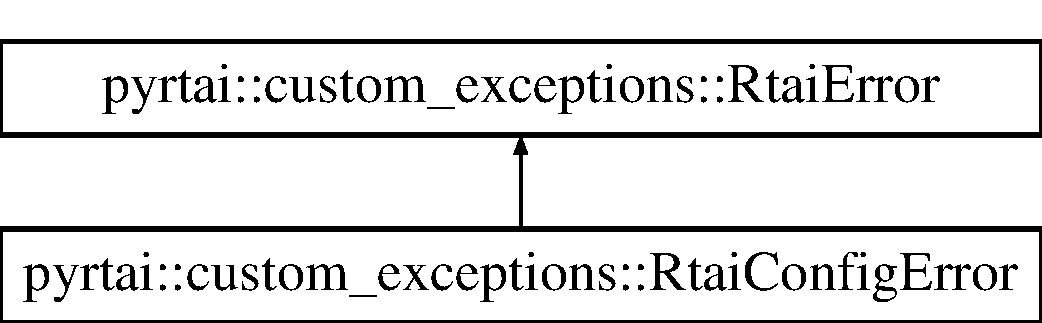
\includegraphics[height=2.000000cm]{classpyrtai_1_1custom__exceptions_1_1_rtai_config_error}
\end{center}
\end{figure}
\subsection*{\-Public \-Member \-Functions}
\begin{DoxyCompactItemize}
\item 
def \hyperlink{classpyrtai_1_1custom__exceptions_1_1_rtai_config_error_a91d26510a3e36cc429380781cde015c0}{\-\_\-\-\_\-init\-\_\-\-\_\-}
\begin{DoxyCompactList}\small\item\em \-Saves expr and msg of the error. \end{DoxyCompactList}\item 
def \hyperlink{classpyrtai_1_1custom__exceptions_1_1_rtai_config_error_a2cf33638d1e2c3f4299ae7e220713f33}{\-\_\-\-\_\-str\-\_\-\-\_\-}
\begin{DoxyCompactList}\small\item\em \-Returns string representation of the error. \end{DoxyCompactList}\end{DoxyCompactItemize}
\subsection*{\-Public \-Attributes}
\begin{DoxyCompactItemize}
\item 
\hyperlink{classpyrtai_1_1custom__exceptions_1_1_rtai_config_error_aa12b3a8f9559dae949056c77839f3264}{expr}
\begin{DoxyCompactList}\small\item\em \-Input expression in which the error occurred. \end{DoxyCompactList}\item 
\hyperlink{classpyrtai_1_1custom__exceptions_1_1_rtai_config_error_a55d1fa78a1ddc2d19f702e92566d65ce}{msg}
\begin{DoxyCompactList}\small\item\em \-Explanation of the error. \end{DoxyCompactList}\end{DoxyCompactItemize}


\subsection{\-Detailed \-Description}
\-Exception raised for errors involving connections. 

\subsection{\-Constructor \& \-Destructor \-Documentation}
\hypertarget{classpyrtai_1_1custom__exceptions_1_1_rtai_config_error_a91d26510a3e36cc429380781cde015c0}{
\index{pyrtai\-::custom\-\_\-exceptions\-::\-Rtai\-Config\-Error@{pyrtai\-::custom\-\_\-exceptions\-::\-Rtai\-Config\-Error}!\-\_\-\-\_\-init\-\_\-\-\_\-@{\-\_\-\-\_\-init\-\_\-\-\_\-}}
\index{\-\_\-\-\_\-init\-\_\-\-\_\-@{\-\_\-\-\_\-init\-\_\-\-\_\-}!pyrtai::custom_exceptions::RtaiConfigError@{pyrtai\-::custom\-\_\-exceptions\-::\-Rtai\-Config\-Error}}
\subsubsection[{\-\_\-\-\_\-init\-\_\-\-\_\-}]{\setlength{\rightskip}{0pt plus 5cm}def pyrtai\-::custom\-\_\-exceptions\-::\-Rtai\-Config\-Error\-::\-\_\-\-\_\-init\-\_\-\-\_\- (
\begin{DoxyParamCaption}
\item[{}]{self, }
\item[{}]{expr, }
\item[{}]{msg}
\end{DoxyParamCaption}
)}}
\label{classpyrtai_1_1custom__exceptions_1_1_rtai_config_error_a91d26510a3e36cc429380781cde015c0}


\-Saves expr and msg of the error. 



\-Definition at line 18 of file custom\-\_\-exceptions.\-py.



\subsection{\-Member \-Function \-Documentation}
\hypertarget{classpyrtai_1_1custom__exceptions_1_1_rtai_config_error_a2cf33638d1e2c3f4299ae7e220713f33}{
\index{pyrtai\-::custom\-\_\-exceptions\-::\-Rtai\-Config\-Error@{pyrtai\-::custom\-\_\-exceptions\-::\-Rtai\-Config\-Error}!\-\_\-\-\_\-str\-\_\-\-\_\-@{\-\_\-\-\_\-str\-\_\-\-\_\-}}
\index{\-\_\-\-\_\-str\-\_\-\-\_\-@{\-\_\-\-\_\-str\-\_\-\-\_\-}!pyrtai::custom_exceptions::RtaiConfigError@{pyrtai\-::custom\-\_\-exceptions\-::\-Rtai\-Config\-Error}}
\subsubsection[{\-\_\-\-\_\-str\-\_\-\-\_\-}]{\setlength{\rightskip}{0pt plus 5cm}def pyrtai\-::custom\-\_\-exceptions\-::\-Rtai\-Config\-Error\-::\-\_\-\-\_\-str\-\_\-\-\_\- (
\begin{DoxyParamCaption}
\item[{}]{self}
\end{DoxyParamCaption}
)}}
\label{classpyrtai_1_1custom__exceptions_1_1_rtai_config_error_a2cf33638d1e2c3f4299ae7e220713f33}


\-Returns string representation of the error. 



\-Definition at line 23 of file custom\-\_\-exceptions.\-py.



\subsection{\-Member \-Data \-Documentation}
\hypertarget{classpyrtai_1_1custom__exceptions_1_1_rtai_config_error_aa12b3a8f9559dae949056c77839f3264}{
\index{pyrtai\-::custom\-\_\-exceptions\-::\-Rtai\-Config\-Error@{pyrtai\-::custom\-\_\-exceptions\-::\-Rtai\-Config\-Error}!expr@{expr}}
\index{expr@{expr}!pyrtai::custom_exceptions::RtaiConfigError@{pyrtai\-::custom\-\_\-exceptions\-::\-Rtai\-Config\-Error}}
\subsubsection[{expr}]{\setlength{\rightskip}{0pt plus 5cm}{\bf pyrtai\-::custom\-\_\-exceptions\-::\-Rtai\-Config\-Error\-::expr}}}
\label{classpyrtai_1_1custom__exceptions_1_1_rtai_config_error_aa12b3a8f9559dae949056c77839f3264}


\-Input expression in which the error occurred. 



\-Definition at line 18 of file custom\-\_\-exceptions.\-py.

\hypertarget{classpyrtai_1_1custom__exceptions_1_1_rtai_config_error_a55d1fa78a1ddc2d19f702e92566d65ce}{
\index{pyrtai\-::custom\-\_\-exceptions\-::\-Rtai\-Config\-Error@{pyrtai\-::custom\-\_\-exceptions\-::\-Rtai\-Config\-Error}!msg@{msg}}
\index{msg@{msg}!pyrtai::custom_exceptions::RtaiConfigError@{pyrtai\-::custom\-\_\-exceptions\-::\-Rtai\-Config\-Error}}
\subsubsection[{msg}]{\setlength{\rightskip}{0pt plus 5cm}{\bf pyrtai\-::custom\-\_\-exceptions\-::\-Rtai\-Config\-Error\-::msg}}}
\label{classpyrtai_1_1custom__exceptions_1_1_rtai_config_error_a55d1fa78a1ddc2d19f702e92566d65ce}


\-Explanation of the error. 



\-Definition at line 18 of file custom\-\_\-exceptions.\-py.



\-The documentation for this class was generated from the following file\-:\begin{DoxyCompactItemize}
\item 
/home/drwolf/\-Devel/py\-R\-T\-A\-I/pyrtai/\hyperlink{custom__exceptions_8py}{custom\-\_\-exceptions.\-py}\end{DoxyCompactItemize}

\hypertarget{classpyrtai_1_1custom__exceptions_1_1_rtai_error}{
\section{pyrtai\-:\-:custom\-\_\-exceptions\-:\-:\-Rtai\-Error \-Class \-Reference}
\label{classpyrtai_1_1custom__exceptions_1_1_rtai_error}\index{pyrtai\-::custom\-\_\-exceptions\-::\-Rtai\-Error@{pyrtai\-::custom\-\_\-exceptions\-::\-Rtai\-Error}}
}


\-Base class for exceptions in this module.  


\-Inheritance diagram for pyrtai\-:\-:custom\-\_\-exceptions\-:\-:\-Rtai\-Error\-:\begin{figure}[H]
\begin{center}
\leavevmode
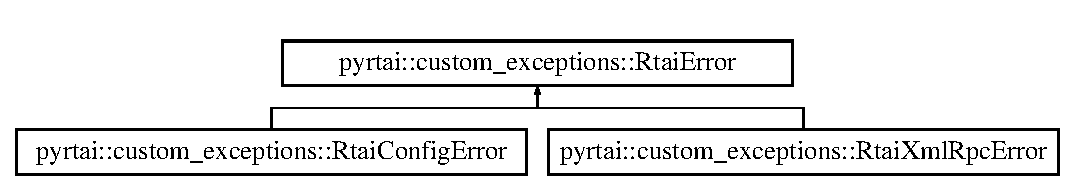
\includegraphics[height=2.000000cm]{classpyrtai_1_1custom__exceptions_1_1_rtai_error}
\end{center}
\end{figure}


\subsection{\-Detailed \-Description}
\-Base class for exceptions in this module. 

\-The documentation for this class was generated from the following file\-:\begin{DoxyCompactItemize}
\item 
/home/drwolf/\-Devel/py\-R\-T\-A\-I/pyrtai/\hyperlink{custom__exceptions_8py}{custom\-\_\-exceptions.\-py}\end{DoxyCompactItemize}

\hypertarget{classpyrtai_1_1rtai__server_1_1_rtai_server}{
\section{pyrtai\-:\-:rtai\-\_\-server\-:\-:\-Rtai\-Server \-Class \-Reference}
\label{classpyrtai_1_1rtai__server_1_1_rtai_server}\index{pyrtai\-::rtai\-\_\-server\-::\-Rtai\-Server@{pyrtai\-::rtai\-\_\-server\-::\-Rtai\-Server}}
}
\subsection*{\-Public \-Member \-Functions}
\begin{DoxyCompactItemize}
\item 
def \hyperlink{classpyrtai_1_1rtai__server_1_1_rtai_server_a007e1e53170de1e75e6d0561fdbeec70}{\-\_\-\-\_\-init\-\_\-\-\_\-}
\begin{DoxyCompactList}\small\item\em \hyperlink{classpyrtai_1_1rtai__server_1_1_rtai_server}{\-Rtai\-Server} initializer. \end{DoxyCompactList}\item 
def \hyperlink{classpyrtai_1_1rtai__server_1_1_rtai_server_a09adc29cacb9005385e0408ef44aa698}{get\-Target}
\begin{DoxyCompactList}\small\item\em \-Creates the target \-If the first connection, it connects to master, then to the slave. \end{DoxyCompactList}\item 
def \hyperlink{classpyrtai_1_1rtai__server_1_1_rtai_server_a55d330bcb7d996b6417018c7462d9e11}{halt}
\begin{DoxyCompactList}\small\item\em \-Stops everything. \end{DoxyCompactList}\end{DoxyCompactItemize}
\subsection*{\-Public \-Attributes}
\begin{DoxyCompactItemize}
\item 
\hyperlink{classpyrtai_1_1rtai__server_1_1_rtai_server_a21c21afe6f0d580bcbe5f3dff9b5b2db}{master}
\begin{DoxyCompactList}\small\item\em \-The master \-R\-T\-A\-I-\/\-X\-M\-L server. \end{DoxyCompactList}\item 
\hyperlink{classpyrtai_1_1rtai__server_1_1_rtai_server_a5ba04b29d8f31daf8ad004d755f35c2c}{slave}
\begin{DoxyCompactList}\small\item\em \-The slave \-R\-T\-A\-I-\/\-X\-M\-L server. \end{DoxyCompactList}\item 
\hyperlink{classpyrtai_1_1rtai__server_1_1_rtai_server_a73a84c2d529fa4c391b063a12f3e728c}{protocol}
\begin{DoxyCompactList}\small\item\em \-The protocol to use to connect to the server (http$|$https) \end{DoxyCompactList}\item 
\hyperlink{classpyrtai_1_1rtai__server_1_1_rtai_server_a2353509bf09ba99d461716173f876fcf}{address}
\begin{DoxyCompactList}\small\item\em \-The address of the server. \end{DoxyCompactList}\item 
\hyperlink{classpyrtai_1_1rtai__server_1_1_rtai_server_a37a7acb27c10fbdb822e2dadc8284908}{port}
\begin{DoxyCompactList}\small\item\em \-The port to use on the server. \end{DoxyCompactList}\item 
\hyperlink{classpyrtai_1_1rtai__server_1_1_rtai_server_af609c8237aab35aeec077d8e198dbf4d}{target\-\_\-name}
\begin{DoxyCompactList}\small\item\em \-The target name to connect to. \end{DoxyCompactList}\end{DoxyCompactItemize}


\subsection{\-Constructor \& \-Destructor \-Documentation}
\hypertarget{classpyrtai_1_1rtai__server_1_1_rtai_server_a007e1e53170de1e75e6d0561fdbeec70}{
\index{pyrtai\-::rtai\-\_\-server\-::\-Rtai\-Server@{pyrtai\-::rtai\-\_\-server\-::\-Rtai\-Server}!\-\_\-\-\_\-init\-\_\-\-\_\-@{\-\_\-\-\_\-init\-\_\-\-\_\-}}
\index{\-\_\-\-\_\-init\-\_\-\-\_\-@{\-\_\-\-\_\-init\-\_\-\-\_\-}!pyrtai::rtai_server::RtaiServer@{pyrtai\-::rtai\-\_\-server\-::\-Rtai\-Server}}
\subsubsection[{\-\_\-\-\_\-init\-\_\-\-\_\-}]{\setlength{\rightskip}{0pt plus 5cm}def pyrtai\-::rtai\-\_\-server\-::\-Rtai\-Server\-::\-\_\-\-\_\-init\-\_\-\-\_\- (
\begin{DoxyParamCaption}
\item[{}]{self, }
\item[{}]{target\-\_\-name = {\ttfamily \-None}, }
\item[{}]{protocol = {\ttfamily \-None}, }
\item[{}]{address = {\ttfamily \-None}, }
\item[{}]{port = {\ttfamily \-None}}
\end{DoxyParamCaption}
)}}
\label{classpyrtai_1_1rtai__server_1_1_rtai_server_a007e1e53170de1e75e6d0561fdbeec70}


\hyperlink{classpyrtai_1_1rtai__server_1_1_rtai_server}{\-Rtai\-Server} initializer. 

\-If the params are \-None, they're extracted from self.\-configurator when the \-Target is created 
\begin{DoxyParams}{\-Parameters}
{\em target\-\_\-name} & \-The target name to connect to (\-T\-O\-D\-O\-: e' lo script name, non il targe name) \\
\hline
{\em protocol} & \-The protocol to use to connect to the server (http$|$https) \\
\hline
{\em address} & \-The address of the server \\
\hline
{\em port} & \-The port to use on the server \\
\hline
\end{DoxyParams}


\-Definition at line 32 of file rtai\-\_\-server.\-py.



\subsection{\-Member \-Function \-Documentation}
\hypertarget{classpyrtai_1_1rtai__server_1_1_rtai_server_a09adc29cacb9005385e0408ef44aa698}{
\index{pyrtai\-::rtai\-\_\-server\-::\-Rtai\-Server@{pyrtai\-::rtai\-\_\-server\-::\-Rtai\-Server}!get\-Target@{get\-Target}}
\index{get\-Target@{get\-Target}!pyrtai::rtai_server::RtaiServer@{pyrtai\-::rtai\-\_\-server\-::\-Rtai\-Server}}
\subsubsection[{get\-Target}]{\setlength{\rightskip}{0pt plus 5cm}def pyrtai\-::rtai\-\_\-server\-::\-Rtai\-Server\-::get\-Target (
\begin{DoxyParamCaption}
\item[{}]{self, }
\item[{}]{target\-\_\-name = {\ttfamily \-None}, }
\item[{}]{password = {\ttfamily \-None}}
\end{DoxyParamCaption}
)}}
\label{classpyrtai_1_1rtai__server_1_1_rtai_server_a09adc29cacb9005385e0408ef44aa698}


\-Creates the target \-If the first connection, it connects to master, then to the slave. 

\-If a slave\-\_\-target param is passed, it connects to the specified target 
\begin{DoxyParams}{\-Parameters}
{\em target\-\_\-name} & \-The target to connect to. \-Can be \-None to request a standard slave target \\
\hline
{\em password} & \-The master password to catch a running server \\
\hline
\end{DoxyParams}
\begin{DoxyReturn}{\-Returns}
\-The connected target. \-False if an error occurs (the error message is printed) 
\end{DoxyReturn}


\-Definition at line 46 of file rtai\-\_\-server.\-py.

\hypertarget{classpyrtai_1_1rtai__server_1_1_rtai_server_a55d330bcb7d996b6417018c7462d9e11}{
\index{pyrtai\-::rtai\-\_\-server\-::\-Rtai\-Server@{pyrtai\-::rtai\-\_\-server\-::\-Rtai\-Server}!halt@{halt}}
\index{halt@{halt}!pyrtai::rtai_server::RtaiServer@{pyrtai\-::rtai\-\_\-server\-::\-Rtai\-Server}}
\subsubsection[{halt}]{\setlength{\rightskip}{0pt plus 5cm}def pyrtai\-::rtai\-\_\-server\-::\-Rtai\-Server\-::halt (
\begin{DoxyParamCaption}
\item[{}]{self}
\end{DoxyParamCaption}
)}}
\label{classpyrtai_1_1rtai__server_1_1_rtai_server_a55d330bcb7d996b6417018c7462d9e11}


\-Stops everything. 



\-Definition at line 76 of file rtai\-\_\-server.\-py.



\subsection{\-Member \-Data \-Documentation}
\hypertarget{classpyrtai_1_1rtai__server_1_1_rtai_server_a2353509bf09ba99d461716173f876fcf}{
\index{pyrtai\-::rtai\-\_\-server\-::\-Rtai\-Server@{pyrtai\-::rtai\-\_\-server\-::\-Rtai\-Server}!address@{address}}
\index{address@{address}!pyrtai::rtai_server::RtaiServer@{pyrtai\-::rtai\-\_\-server\-::\-Rtai\-Server}}
\subsubsection[{address}]{\setlength{\rightskip}{0pt plus 5cm}{\bf pyrtai\-::rtai\-\_\-server\-::\-Rtai\-Server\-::address}}}
\label{classpyrtai_1_1rtai__server_1_1_rtai_server_a2353509bf09ba99d461716173f876fcf}


\-The address of the server. 



\-Definition at line 32 of file rtai\-\_\-server.\-py.

\hypertarget{classpyrtai_1_1rtai__server_1_1_rtai_server_a21c21afe6f0d580bcbe5f3dff9b5b2db}{
\index{pyrtai\-::rtai\-\_\-server\-::\-Rtai\-Server@{pyrtai\-::rtai\-\_\-server\-::\-Rtai\-Server}!master@{master}}
\index{master@{master}!pyrtai::rtai_server::RtaiServer@{pyrtai\-::rtai\-\_\-server\-::\-Rtai\-Server}}
\subsubsection[{master}]{\setlength{\rightskip}{0pt plus 5cm}{\bf pyrtai\-::rtai\-\_\-server\-::\-Rtai\-Server\-::master}}}
\label{classpyrtai_1_1rtai__server_1_1_rtai_server_a21c21afe6f0d580bcbe5f3dff9b5b2db}


\-The master \-R\-T\-A\-I-\/\-X\-M\-L server. 



\-Definition at line 32 of file rtai\-\_\-server.\-py.

\hypertarget{classpyrtai_1_1rtai__server_1_1_rtai_server_a37a7acb27c10fbdb822e2dadc8284908}{
\index{pyrtai\-::rtai\-\_\-server\-::\-Rtai\-Server@{pyrtai\-::rtai\-\_\-server\-::\-Rtai\-Server}!port@{port}}
\index{port@{port}!pyrtai::rtai_server::RtaiServer@{pyrtai\-::rtai\-\_\-server\-::\-Rtai\-Server}}
\subsubsection[{port}]{\setlength{\rightskip}{0pt plus 5cm}{\bf pyrtai\-::rtai\-\_\-server\-::\-Rtai\-Server\-::port}}}
\label{classpyrtai_1_1rtai__server_1_1_rtai_server_a37a7acb27c10fbdb822e2dadc8284908}


\-The port to use on the server. 



\-Definition at line 32 of file rtai\-\_\-server.\-py.

\hypertarget{classpyrtai_1_1rtai__server_1_1_rtai_server_a73a84c2d529fa4c391b063a12f3e728c}{
\index{pyrtai\-::rtai\-\_\-server\-::\-Rtai\-Server@{pyrtai\-::rtai\-\_\-server\-::\-Rtai\-Server}!protocol@{protocol}}
\index{protocol@{protocol}!pyrtai::rtai_server::RtaiServer@{pyrtai\-::rtai\-\_\-server\-::\-Rtai\-Server}}
\subsubsection[{protocol}]{\setlength{\rightskip}{0pt plus 5cm}{\bf pyrtai\-::rtai\-\_\-server\-::\-Rtai\-Server\-::protocol}}}
\label{classpyrtai_1_1rtai__server_1_1_rtai_server_a73a84c2d529fa4c391b063a12f3e728c}


\-The protocol to use to connect to the server (http$|$https) 



\-Definition at line 32 of file rtai\-\_\-server.\-py.

\hypertarget{classpyrtai_1_1rtai__server_1_1_rtai_server_a5ba04b29d8f31daf8ad004d755f35c2c}{
\index{pyrtai\-::rtai\-\_\-server\-::\-Rtai\-Server@{pyrtai\-::rtai\-\_\-server\-::\-Rtai\-Server}!slave@{slave}}
\index{slave@{slave}!pyrtai::rtai_server::RtaiServer@{pyrtai\-::rtai\-\_\-server\-::\-Rtai\-Server}}
\subsubsection[{slave}]{\setlength{\rightskip}{0pt plus 5cm}{\bf pyrtai\-::rtai\-\_\-server\-::\-Rtai\-Server\-::slave}}}
\label{classpyrtai_1_1rtai__server_1_1_rtai_server_a5ba04b29d8f31daf8ad004d755f35c2c}


\-The slave \-R\-T\-A\-I-\/\-X\-M\-L server. 



\-Definition at line 32 of file rtai\-\_\-server.\-py.

\hypertarget{classpyrtai_1_1rtai__server_1_1_rtai_server_af609c8237aab35aeec077d8e198dbf4d}{
\index{pyrtai\-::rtai\-\_\-server\-::\-Rtai\-Server@{pyrtai\-::rtai\-\_\-server\-::\-Rtai\-Server}!target\-\_\-name@{target\-\_\-name}}
\index{target\-\_\-name@{target\-\_\-name}!pyrtai::rtai_server::RtaiServer@{pyrtai\-::rtai\-\_\-server\-::\-Rtai\-Server}}
\subsubsection[{target\-\_\-name}]{\setlength{\rightskip}{0pt plus 5cm}{\bf pyrtai\-::rtai\-\_\-server\-::\-Rtai\-Server\-::target\-\_\-name}}}
\label{classpyrtai_1_1rtai__server_1_1_rtai_server_af609c8237aab35aeec077d8e198dbf4d}


\-The target name to connect to. 



\-Definition at line 32 of file rtai\-\_\-server.\-py.



\-The documentation for this class was generated from the following file\-:\begin{DoxyCompactItemize}
\item 
/home/drwolf/\-Devel/py\-R\-T\-A\-I/pyrtai/\hyperlink{rtai__server_8py}{rtai\-\_\-server.\-py}\end{DoxyCompactItemize}

\hypertarget{classpyrtai_1_1custom__exceptions_1_1_rtai_xml_rpc_error}{
\section{pyrtai\-:\-:custom\-\_\-exceptions\-:\-:\-Rtai\-Xml\-Rpc\-Error \-Class \-Reference}
\label{classpyrtai_1_1custom__exceptions_1_1_rtai_xml_rpc_error}\index{pyrtai\-::custom\-\_\-exceptions\-::\-Rtai\-Xml\-Rpc\-Error@{pyrtai\-::custom\-\_\-exceptions\-::\-Rtai\-Xml\-Rpc\-Error}}
}


\-Exception raised for errors involving connections.  


\-Inheritance diagram for pyrtai\-:\-:custom\-\_\-exceptions\-:\-:\-Rtai\-Xml\-Rpc\-Error\-:\begin{figure}[H]
\begin{center}
\leavevmode
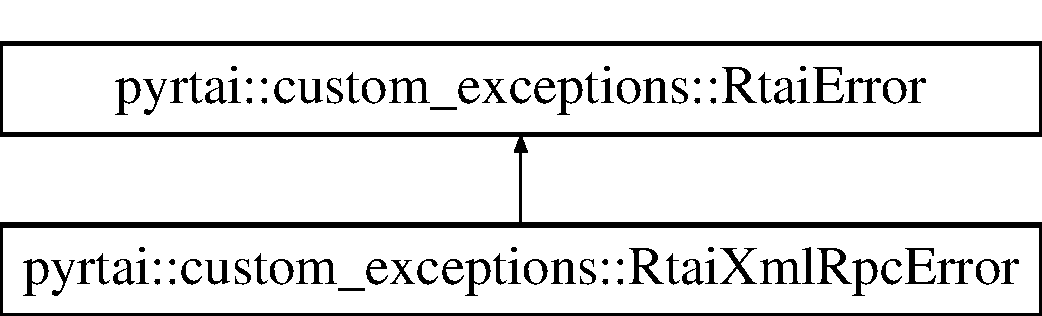
\includegraphics[height=2.000000cm]{classpyrtai_1_1custom__exceptions_1_1_rtai_xml_rpc_error}
\end{center}
\end{figure}
\subsection*{\-Public \-Member \-Functions}
\begin{DoxyCompactItemize}
\item 
def \hyperlink{classpyrtai_1_1custom__exceptions_1_1_rtai_xml_rpc_error_af7e7292eb31393297fecb648f4a24dfb}{\-\_\-\-\_\-init\-\_\-\-\_\-}
\begin{DoxyCompactList}\small\item\em \-Saves expr and msg of the error. \end{DoxyCompactList}\item 
def \hyperlink{classpyrtai_1_1custom__exceptions_1_1_rtai_xml_rpc_error_a3c85aadda9365580b03d849e30b6c554}{\-\_\-\-\_\-str\-\_\-\-\_\-}
\begin{DoxyCompactList}\small\item\em \-Returns string representation of the error. \end{DoxyCompactList}\end{DoxyCompactItemize}
\subsection*{\-Public \-Attributes}
\begin{DoxyCompactItemize}
\item 
\hyperlink{classpyrtai_1_1custom__exceptions_1_1_rtai_xml_rpc_error_aff73970aa9888d169959f1a49e59730d}{expr}
\begin{DoxyCompactList}\small\item\em \-Input expression in which the error occurred. \end{DoxyCompactList}\item 
\hyperlink{classpyrtai_1_1custom__exceptions_1_1_rtai_xml_rpc_error_ae27d2ff28611a7af8703c3ee90e224a3}{msg}
\begin{DoxyCompactList}\small\item\em \-Explanation of the error. \end{DoxyCompactList}\end{DoxyCompactItemize}


\subsection{\-Detailed \-Description}
\-Exception raised for errors involving connections. 

\subsection{\-Constructor \& \-Destructor \-Documentation}
\hypertarget{classpyrtai_1_1custom__exceptions_1_1_rtai_xml_rpc_error_af7e7292eb31393297fecb648f4a24dfb}{
\index{pyrtai\-::custom\-\_\-exceptions\-::\-Rtai\-Xml\-Rpc\-Error@{pyrtai\-::custom\-\_\-exceptions\-::\-Rtai\-Xml\-Rpc\-Error}!\-\_\-\-\_\-init\-\_\-\-\_\-@{\-\_\-\-\_\-init\-\_\-\-\_\-}}
\index{\-\_\-\-\_\-init\-\_\-\-\_\-@{\-\_\-\-\_\-init\-\_\-\-\_\-}!pyrtai::custom_exceptions::RtaiXmlRpcError@{pyrtai\-::custom\-\_\-exceptions\-::\-Rtai\-Xml\-Rpc\-Error}}
\subsubsection[{\-\_\-\-\_\-init\-\_\-\-\_\-}]{\setlength{\rightskip}{0pt plus 5cm}def pyrtai\-::custom\-\_\-exceptions\-::\-Rtai\-Xml\-Rpc\-Error\-::\-\_\-\-\_\-init\-\_\-\-\_\- (
\begin{DoxyParamCaption}
\item[{}]{self, }
\item[{}]{expr, }
\item[{}]{msg}
\end{DoxyParamCaption}
)}}
\label{classpyrtai_1_1custom__exceptions_1_1_rtai_xml_rpc_error_af7e7292eb31393297fecb648f4a24dfb}


\-Saves expr and msg of the error. 



\-Definition at line 36 of file custom\-\_\-exceptions.\-py.



\subsection{\-Member \-Function \-Documentation}
\hypertarget{classpyrtai_1_1custom__exceptions_1_1_rtai_xml_rpc_error_a3c85aadda9365580b03d849e30b6c554}{
\index{pyrtai\-::custom\-\_\-exceptions\-::\-Rtai\-Xml\-Rpc\-Error@{pyrtai\-::custom\-\_\-exceptions\-::\-Rtai\-Xml\-Rpc\-Error}!\-\_\-\-\_\-str\-\_\-\-\_\-@{\-\_\-\-\_\-str\-\_\-\-\_\-}}
\index{\-\_\-\-\_\-str\-\_\-\-\_\-@{\-\_\-\-\_\-str\-\_\-\-\_\-}!pyrtai::custom_exceptions::RtaiXmlRpcError@{pyrtai\-::custom\-\_\-exceptions\-::\-Rtai\-Xml\-Rpc\-Error}}
\subsubsection[{\-\_\-\-\_\-str\-\_\-\-\_\-}]{\setlength{\rightskip}{0pt plus 5cm}def pyrtai\-::custom\-\_\-exceptions\-::\-Rtai\-Xml\-Rpc\-Error\-::\-\_\-\-\_\-str\-\_\-\-\_\- (
\begin{DoxyParamCaption}
\item[{}]{self}
\end{DoxyParamCaption}
)}}
\label{classpyrtai_1_1custom__exceptions_1_1_rtai_xml_rpc_error_a3c85aadda9365580b03d849e30b6c554}


\-Returns string representation of the error. 



\-Definition at line 41 of file custom\-\_\-exceptions.\-py.



\subsection{\-Member \-Data \-Documentation}
\hypertarget{classpyrtai_1_1custom__exceptions_1_1_rtai_xml_rpc_error_aff73970aa9888d169959f1a49e59730d}{
\index{pyrtai\-::custom\-\_\-exceptions\-::\-Rtai\-Xml\-Rpc\-Error@{pyrtai\-::custom\-\_\-exceptions\-::\-Rtai\-Xml\-Rpc\-Error}!expr@{expr}}
\index{expr@{expr}!pyrtai::custom_exceptions::RtaiXmlRpcError@{pyrtai\-::custom\-\_\-exceptions\-::\-Rtai\-Xml\-Rpc\-Error}}
\subsubsection[{expr}]{\setlength{\rightskip}{0pt plus 5cm}{\bf pyrtai\-::custom\-\_\-exceptions\-::\-Rtai\-Xml\-Rpc\-Error\-::expr}}}
\label{classpyrtai_1_1custom__exceptions_1_1_rtai_xml_rpc_error_aff73970aa9888d169959f1a49e59730d}


\-Input expression in which the error occurred. 



\-Definition at line 36 of file custom\-\_\-exceptions.\-py.

\hypertarget{classpyrtai_1_1custom__exceptions_1_1_rtai_xml_rpc_error_ae27d2ff28611a7af8703c3ee90e224a3}{
\index{pyrtai\-::custom\-\_\-exceptions\-::\-Rtai\-Xml\-Rpc\-Error@{pyrtai\-::custom\-\_\-exceptions\-::\-Rtai\-Xml\-Rpc\-Error}!msg@{msg}}
\index{msg@{msg}!pyrtai::custom_exceptions::RtaiXmlRpcError@{pyrtai\-::custom\-\_\-exceptions\-::\-Rtai\-Xml\-Rpc\-Error}}
\subsubsection[{msg}]{\setlength{\rightskip}{0pt plus 5cm}{\bf pyrtai\-::custom\-\_\-exceptions\-::\-Rtai\-Xml\-Rpc\-Error\-::msg}}}
\label{classpyrtai_1_1custom__exceptions_1_1_rtai_xml_rpc_error_ae27d2ff28611a7af8703c3ee90e224a3}


\-Explanation of the error. 



\-Definition at line 36 of file custom\-\_\-exceptions.\-py.



\-The documentation for this class was generated from the following file\-:\begin{DoxyCompactItemize}
\item 
/home/drwolf/\-Devel/py\-R\-T\-A\-I/pyrtai/\hyperlink{custom__exceptions_8py}{custom\-\_\-exceptions.\-py}\end{DoxyCompactItemize}

\hypertarget{classpyrtai_1_1target_1_1_target}{
\section{pyrtai\-:\-:target\-:\-:\-Target \-Class \-Reference}
\label{classpyrtai_1_1target_1_1_target}\index{pyrtai\-::target\-::\-Target@{pyrtai\-::target\-::\-Target}}
}
\subsection*{\-Public \-Member \-Functions}
\begin{DoxyCompactItemize}
\item 
def \hyperlink{classpyrtai_1_1target_1_1_target_ad89e94e6a5cf413af9ad91dd9b83670b}{\-\_\-\-\_\-init\-\_\-\-\_\-}
\begin{DoxyCompactList}\small\item\em \hyperlink{classpyrtai_1_1target_1_1_target}{\-Target} initializer. \end{DoxyCompactList}\item 
def \hyperlink{classpyrtai_1_1target_1_1_target_a9674793e75bd351e481791b881c0f9da}{get\-Info}
\begin{DoxyCompactList}\small\item\em \-Prints a summary of the target and its status \-T\-O\-D\-O\-: \-Decidere che informazioni restituire. \end{DoxyCompactList}\item 
def \hyperlink{classpyrtai_1_1target_1_1_target_ab0cfc0e5b6ac03cf654879045d7b9a13}{setup\-\_\-data\-\_\-threads}
\begin{DoxyCompactList}\small\item\em \-Setups the queue and the threads needed to read the data stream. \end{DoxyCompactList}\item 
def \hyperlink{classpyrtai_1_1target_1_1_target_ae0dd80c9557257d45fbae2d7d7a18ddf}{stop\-\_\-data\-\_\-threads}
\begin{DoxyCompactList}\small\item\em \-Stops the data threads. \end{DoxyCompactList}\item 
def \hyperlink{classpyrtai_1_1target_1_1_target_a792bae526bddd673ef6e07f4c57930b0}{add\-Observer}
\begin{DoxyCompactList}\small\item\em \-Add a new observer \char`\"{}update\char`\"{} method to the list of observers. \end{DoxyCompactList}\item 
def \hyperlink{classpyrtai_1_1target_1_1_target_abe0602fd40e54c1ff92d7310897072ac}{remove\-Observer}
\begin{DoxyCompactList}\small\item\em \-Removes the observer. \end{DoxyCompactList}\item 
def \hyperlink{classpyrtai_1_1target_1_1_target_a8f84994a13eda611de5dc4dc357ba060}{connect}
\begin{DoxyCompactList}\small\item\em \-Connect to the target server. \end{DoxyCompactList}\item 
def \hyperlink{classpyrtai_1_1target_1_1_target_a55c7fb6e7f872139695fad3be58fe811}{get\-Slave}
\begin{DoxyCompactList}\small\item\em \-Checks if master and if affirmative, returns the slave. \end{DoxyCompactList}\item 
def \hyperlink{classpyrtai_1_1target_1_1_target_a6b88fd3e02bd52f9d9596aecaa15414d}{disconnect}
\begin{DoxyCompactList}\small\item\em \-Disconnects from the \-X\-M\-L-\/\-R\-P\-C server. \end{DoxyCompactList}\item 
def \hyperlink{classpyrtai_1_1target_1_1_target_a7a472990dd9d3b1d7c0d3f2aa63ec7a1}{stop}
\begin{DoxyCompactList}\small\item\em \-Stops target server. \end{DoxyCompactList}\item 
def \hyperlink{classpyrtai_1_1target_1_1_target_a12ad20665782eb0e8eac3ea797fbae57}{close}
\begin{DoxyCompactList}\small\item\em \-Closes the session. \end{DoxyCompactList}\item 
def \hyperlink{classpyrtai_1_1target_1_1_target_a8f2a7582fcb34a5244bb5281b34feb47}{halt}
\begin{DoxyCompactList}\small\item\em \-Stops the target \-This method closes the data threads (if they exist) then closes the session. \end{DoxyCompactList}\item 
def \hyperlink{classpyrtai_1_1target_1_1_target_a9a61f08b90d8512663f2c74545943228}{start}
\begin{DoxyCompactList}\small\item\em \-Starts the connected target. \end{DoxyCompactList}\item 
def \hyperlink{classpyrtai_1_1target_1_1_target_aadaa0ae2a3535637dde24e5a822e50e7}{start\-Data}
\begin{DoxyCompactList}\small\item\em \-Starts data transfer for the specified signal. \end{DoxyCompactList}\item 
def \hyperlink{classpyrtai_1_1target_1_1_target_a3419fad652e47f0e1b6adbd7c2f3c76c}{stop\-Data}
\begin{DoxyCompactList}\small\item\em \-Stops (all) data transfers. \end{DoxyCompactList}\item 
def \hyperlink{classpyrtai_1_1target_1_1_target_ac60d73c462fc3988624a36301e7f885f}{get\-Signal\-Structure}
\begin{DoxyCompactList}\small\item\em \-Get the structure of the signals. \end{DoxyCompactList}\item 
def \hyperlink{classpyrtai_1_1target_1_1_target_a2a8d46776e9b4c03081bb4426d849517}{set\-Parameters}
\begin{DoxyCompactList}\small\item\em \-Sends new parameters to the server. \end{DoxyCompactList}\item 
def \hyperlink{classpyrtai_1_1target_1_1_target_a5f5a51ab29bf80e6ff26074e15af49f2}{get\-Parameters}
\begin{DoxyCompactList}\small\item\em \-Get the parameters from the target server. \end{DoxyCompactList}\item 
def \hyperlink{classpyrtai_1_1target_1_1_target_a9d6334d4c1ada8dae518f56ccf8fddab}{set\-Param}
\begin{DoxyCompactList}\small\item\em \-Interface to set a single param. \end{DoxyCompactList}\end{DoxyCompactItemize}
\subsection*{\-Public \-Attributes}
\begin{DoxyCompactItemize}
\item 
\hyperlink{classpyrtai_1_1target_1_1_target_a81312c5e774f702d956b5e21f76b8d48}{config}
\begin{DoxyCompactList}\small\item\em \-A \hyperlink{classpyrtai_1_1configurator_1_1_configurator}{configurator\-::\-Configurator} object. \end{DoxyCompactList}\item 
\hyperlink{classpyrtai_1_1target_1_1_target_a615b77c2475db26f9055078ab7f15f75}{is\-\_\-connected}
\begin{DoxyCompactList}\small\item\em \-Checks if the \hyperlink{classpyrtai_1_1target_1_1_target}{\-Target} is connected or not. \end{DoxyCompactList}\item 
\hyperlink{classpyrtai_1_1target_1_1_target_a38d056a202885bac1459328108d600fa}{is\-\_\-slave}
\begin{DoxyCompactList}\small\item\em \-Shows if this is a slave target. \end{DoxyCompactList}\item 
\hyperlink{classpyrtai_1_1target_1_1_target_aae04036f71a3a512b5461bf97692e7e9}{parameters}
\begin{DoxyCompactList}\small\item\em \-The target parameters. \end{DoxyCompactList}\item 
\hyperlink{classpyrtai_1_1target_1_1_target_a0d458e6387a385c285b33a87e645caee}{datastream\-\_\-queue}
\begin{DoxyCompactList}\small\item\em \-The queue where \-Data\-Collector thread puts data and observers get it. \end{DoxyCompactList}\item 
\hyperlink{classpyrtai_1_1target_1_1_target_a6f53ef231f9caced4bc8ee94404f4550}{datastream\-\_\-poller}
\begin{DoxyCompactList}\small\item\em \-The \-Data\-Poller thread. \end{DoxyCompactList}\item 
\hyperlink{classpyrtai_1_1target_1_1_target_a2e3d692af2e90764b0835991cf538568}{datastream\-\_\-collector}
\begin{DoxyCompactList}\small\item\em \-The \-Data\-Collector thread. \end{DoxyCompactList}\item 
\hyperlink{classpyrtai_1_1target_1_1_target_ab10614e38c19644cfbd81ec3424df5c7}{connection}
\begin{DoxyCompactList}\small\item\em \-A \hyperlink{classpyrtai_1_1connector_1_1_connector}{connector\-::\-Connector} instance used to send commands to \-X\-M\-L-\/\-R\-P\-C connection. \end{DoxyCompactList}\end{DoxyCompactItemize}


\subsection{\-Constructor \& \-Destructor \-Documentation}
\hypertarget{classpyrtai_1_1target_1_1_target_ad89e94e6a5cf413af9ad91dd9b83670b}{
\index{pyrtai\-::target\-::\-Target@{pyrtai\-::target\-::\-Target}!\-\_\-\-\_\-init\-\_\-\-\_\-@{\-\_\-\-\_\-init\-\_\-\-\_\-}}
\index{\-\_\-\-\_\-init\-\_\-\-\_\-@{\-\_\-\-\_\-init\-\_\-\-\_\-}!pyrtai::target::Target@{pyrtai\-::target\-::\-Target}}
\subsubsection[{\-\_\-\-\_\-init\-\_\-\-\_\-}]{\setlength{\rightskip}{0pt plus 5cm}def pyrtai\-::target\-::\-Target\-::\-\_\-\-\_\-init\-\_\-\-\_\- (
\begin{DoxyParamCaption}
\item[{}]{self, }
\item[{}]{slave = {\ttfamily \-False}, }
\item[{}]{protocol = {\ttfamily \-None}, }
\item[{}]{address = {\ttfamily \-None}, }
\item[{}]{port = {\ttfamily \-None}, }
\item[{}]{target\-\_\-name = {\ttfamily \-None}}
\end{DoxyParamCaption}
)}}
\label{classpyrtai_1_1target_1_1_target_ad89e94e6a5cf413af9ad91dd9b83670b}


\hyperlink{classpyrtai_1_1target_1_1_target}{\-Target} initializer. 



\-Definition at line 37 of file target.\-py.



\subsection{\-Member \-Function \-Documentation}
\hypertarget{classpyrtai_1_1target_1_1_target_a792bae526bddd673ef6e07f4c57930b0}{
\index{pyrtai\-::target\-::\-Target@{pyrtai\-::target\-::\-Target}!add\-Observer@{add\-Observer}}
\index{add\-Observer@{add\-Observer}!pyrtai::target::Target@{pyrtai\-::target\-::\-Target}}
\subsubsection[{add\-Observer}]{\setlength{\rightskip}{0pt plus 5cm}def pyrtai\-::target\-::\-Target\-::add\-Observer (
\begin{DoxyParamCaption}
\item[{}]{self, }
\item[{}]{update\-\_\-method, }
\item[{}]{sample\-\_\-time, }
\item[{}]{decimation = {\ttfamily \-None}, }
\item[{}]{channel = {\ttfamily \-None}}
\end{DoxyParamCaption}
)}}
\label{classpyrtai_1_1target_1_1_target_a792bae526bddd673ef6e07f4c57930b0}


\-Add a new observer \char`\"{}update\char`\"{} method to the list of observers. 


\begin{DoxyParams}{\-Parameters}
{\em update\-\_\-method} & \-Is the method of the observer which will be called when new data arrives. \-The method name is arbitrary, but it must accept a string parameter \\
\hline
{\em channel} & \-The optional channel to register the observer to \\
\hline
{\em sample\-\_\-time} & \-The sample time of the signal \\
\hline
{\em decimation} & \-The decimation to use \\
\hline
\end{DoxyParams}
\begin{DoxyReturn}{\-Returns}
\-The \-I\-D of the observer, to be used to remove the observer 
\end{DoxyReturn}


\-Definition at line 134 of file target.\-py.

\hypertarget{classpyrtai_1_1target_1_1_target_a12ad20665782eb0e8eac3ea797fbae57}{
\index{pyrtai\-::target\-::\-Target@{pyrtai\-::target\-::\-Target}!close@{close}}
\index{close@{close}!pyrtai::target::Target@{pyrtai\-::target\-::\-Target}}
\subsubsection[{close}]{\setlength{\rightskip}{0pt plus 5cm}def pyrtai\-::target\-::\-Target\-::close (
\begin{DoxyParamCaption}
\item[{}]{self}
\end{DoxyParamCaption}
)}}
\label{classpyrtai_1_1target_1_1_target_a12ad20665782eb0e8eac3ea797fbae57}


\-Closes the session. 

\begin{DoxyReturn}{\-Returns}
\-The boolean result of the operation 
\end{DoxyReturn}


\-Definition at line 204 of file target.\-py.

\hypertarget{classpyrtai_1_1target_1_1_target_a8f84994a13eda611de5dc4dc357ba060}{
\index{pyrtai\-::target\-::\-Target@{pyrtai\-::target\-::\-Target}!connect@{connect}}
\index{connect@{connect}!pyrtai::target::Target@{pyrtai\-::target\-::\-Target}}
\subsubsection[{connect}]{\setlength{\rightskip}{0pt plus 5cm}def pyrtai\-::target\-::\-Target\-::connect (
\begin{DoxyParamCaption}
\item[{}]{self, }
\item[{}]{password = {\ttfamily \-None}}
\end{DoxyParamCaption}
)}}
\label{classpyrtai_1_1target_1_1_target_a8f84994a13eda611de5dc4dc357ba060}


\-Connect to the target server. 

\-Checks if master or server and call the right method on \hyperlink{classpyrtai_1_1connector_1_1_connector}{connector\-::\-Connector} 
\begin{DoxyParams}{\-Parameters}
{\em password} & \-The (optional) password to catch a running master connection \\
\hline
\end{DoxyParams}
\begin{DoxyReturn}{\-Returns}
\-The boolean result of the operation 
\end{DoxyReturn}


\-Definition at line 147 of file target.\-py.

\hypertarget{classpyrtai_1_1target_1_1_target_a6b88fd3e02bd52f9d9596aecaa15414d}{
\index{pyrtai\-::target\-::\-Target@{pyrtai\-::target\-::\-Target}!disconnect@{disconnect}}
\index{disconnect@{disconnect}!pyrtai::target::Target@{pyrtai\-::target\-::\-Target}}
\subsubsection[{disconnect}]{\setlength{\rightskip}{0pt plus 5cm}def pyrtai\-::target\-::\-Target\-::disconnect (
\begin{DoxyParamCaption}
\item[{}]{self}
\end{DoxyParamCaption}
)}}
\label{classpyrtai_1_1target_1_1_target_a6b88fd3e02bd52f9d9596aecaa15414d}


\-Disconnects from the \-X\-M\-L-\/\-R\-P\-C server. 

\begin{DoxyReturn}{\-Returns}
\-The boolean result of the operation 
\end{DoxyReturn}


\-Definition at line 178 of file target.\-py.

\hypertarget{classpyrtai_1_1target_1_1_target_a9674793e75bd351e481791b881c0f9da}{
\index{pyrtai\-::target\-::\-Target@{pyrtai\-::target\-::\-Target}!get\-Info@{get\-Info}}
\index{get\-Info@{get\-Info}!pyrtai::target::Target@{pyrtai\-::target\-::\-Target}}
\subsubsection[{get\-Info}]{\setlength{\rightskip}{0pt plus 5cm}def pyrtai\-::target\-::\-Target\-::get\-Info (
\begin{DoxyParamCaption}
\item[{}]{self}
\end{DoxyParamCaption}
)}}
\label{classpyrtai_1_1target_1_1_target_a9674793e75bd351e481791b881c0f9da}


\-Prints a summary of the target and its status \-T\-O\-D\-O\-: \-Decidere che informazioni restituire. 



\-Definition at line 64 of file target.\-py.

\hypertarget{classpyrtai_1_1target_1_1_target_a5f5a51ab29bf80e6ff26074e15af49f2}{
\index{pyrtai\-::target\-::\-Target@{pyrtai\-::target\-::\-Target}!get\-Parameters@{get\-Parameters}}
\index{get\-Parameters@{get\-Parameters}!pyrtai::target::Target@{pyrtai\-::target\-::\-Target}}
\subsubsection[{get\-Parameters}]{\setlength{\rightskip}{0pt plus 5cm}def pyrtai\-::target\-::\-Target\-::get\-Parameters (
\begin{DoxyParamCaption}
\item[{}]{self}
\end{DoxyParamCaption}
)}}
\label{classpyrtai_1_1target_1_1_target_a5f5a51ab29bf80e6ff26074e15af49f2}


\-Get the parameters from the target server. 

\begin{DoxyReturn}{\-Returns}
\-An array of params. \-Every param is an hash 
\end{DoxyReturn}


\-Definition at line 261 of file target.\-py.

\hypertarget{classpyrtai_1_1target_1_1_target_ac60d73c462fc3988624a36301e7f885f}{
\index{pyrtai\-::target\-::\-Target@{pyrtai\-::target\-::\-Target}!get\-Signal\-Structure@{get\-Signal\-Structure}}
\index{get\-Signal\-Structure@{get\-Signal\-Structure}!pyrtai::target::Target@{pyrtai\-::target\-::\-Target}}
\subsubsection[{get\-Signal\-Structure}]{\setlength{\rightskip}{0pt plus 5cm}def pyrtai\-::target\-::\-Target\-::get\-Signal\-Structure (
\begin{DoxyParamCaption}
\item[{}]{self}
\end{DoxyParamCaption}
)}}
\label{classpyrtai_1_1target_1_1_target_ac60d73c462fc3988624a36301e7f885f}


\-Get the structure of the signals. 

\begin{DoxyReturn}{\-Returns}
\-The structure of the signals or \-False if the target has no signals 
\end{DoxyReturn}


\-Definition at line 250 of file target.\-py.

\hypertarget{classpyrtai_1_1target_1_1_target_a55c7fb6e7f872139695fad3be58fe811}{
\index{pyrtai\-::target\-::\-Target@{pyrtai\-::target\-::\-Target}!get\-Slave@{get\-Slave}}
\index{get\-Slave@{get\-Slave}!pyrtai::target::Target@{pyrtai\-::target\-::\-Target}}
\subsubsection[{get\-Slave}]{\setlength{\rightskip}{0pt plus 5cm}def pyrtai\-::target\-::\-Target\-::get\-Slave (
\begin{DoxyParamCaption}
\item[{}]{self, }
\item[{}]{target\-\_\-name = {\ttfamily \-None}}
\end{DoxyParamCaption}
)}}
\label{classpyrtai_1_1target_1_1_target_a55c7fb6e7f872139695fad3be58fe811}


\-Checks if master and if affirmative, returns the slave. 


\begin{DoxyParams}{\-Parameters}
{\em target\-\_\-name} & \-The target to connect to. \-If \-None gets the name from the default configuration \\
\hline
\end{DoxyParams}
\begin{DoxyReturn}{\-Returns}
\-The slave \hyperlink{classpyrtai_1_1target_1_1_target}{\-Target} or \-False if not a master target 
\end{DoxyReturn}


\-Definition at line 162 of file target.\-py.

\hypertarget{classpyrtai_1_1target_1_1_target_a8f2a7582fcb34a5244bb5281b34feb47}{
\index{pyrtai\-::target\-::\-Target@{pyrtai\-::target\-::\-Target}!halt@{halt}}
\index{halt@{halt}!pyrtai::target::Target@{pyrtai\-::target\-::\-Target}}
\subsubsection[{halt}]{\setlength{\rightskip}{0pt plus 5cm}def pyrtai\-::target\-::\-Target\-::halt (
\begin{DoxyParamCaption}
\item[{}]{self}
\end{DoxyParamCaption}
)}}
\label{classpyrtai_1_1target_1_1_target_a8f2a7582fcb34a5244bb5281b34feb47}


\-Stops the target \-This method closes the data threads (if they exist) then closes the session. 

\begin{DoxyReturn}{\-Returns}
\-The boolean result of the operation 
\end{DoxyReturn}


\-Definition at line 214 of file target.\-py.

\hypertarget{classpyrtai_1_1target_1_1_target_abe0602fd40e54c1ff92d7310897072ac}{
\index{pyrtai\-::target\-::\-Target@{pyrtai\-::target\-::\-Target}!remove\-Observer@{remove\-Observer}}
\index{remove\-Observer@{remove\-Observer}!pyrtai::target::Target@{pyrtai\-::target\-::\-Target}}
\subsubsection[{remove\-Observer}]{\setlength{\rightskip}{0pt plus 5cm}def pyrtai\-::target\-::\-Target\-::remove\-Observer (
\begin{DoxyParamCaption}
\item[{}]{self, }
\item[{}]{observer\-\_\-id}
\end{DoxyParamCaption}
)}}
\label{classpyrtai_1_1target_1_1_target_abe0602fd40e54c1ff92d7310897072ac}


\-Removes the observer. 


\begin{DoxyParams}{\-Parameters}
{\em observer\-\_\-id} & \-The \-I\-D of the observer to remove \\
\hline
\end{DoxyParams}
\begin{DoxyReturn}{\-Returns}
\-False if the observer isn't in the observers list, \-True if it was correctly removed 
\end{DoxyReturn}


\-Definition at line 141 of file target.\-py.

\hypertarget{classpyrtai_1_1target_1_1_target_a9d6334d4c1ada8dae518f56ccf8fddab}{
\index{pyrtai\-::target\-::\-Target@{pyrtai\-::target\-::\-Target}!set\-Param@{set\-Param}}
\index{set\-Param@{set\-Param}!pyrtai::target::Target@{pyrtai\-::target\-::\-Target}}
\subsubsection[{set\-Param}]{\setlength{\rightskip}{0pt plus 5cm}def pyrtai\-::target\-::\-Target\-::set\-Param (
\begin{DoxyParamCaption}
\item[{}]{self, }
\item[{}]{identifier, }
\item[{}]{value}
\end{DoxyParamCaption}
)}}
\label{classpyrtai_1_1target_1_1_target_a9d6334d4c1ada8dae518f56ccf8fddab}


\-Interface to set a single param. 


\begin{DoxyParams}{\-Parameters}
{\em identifier} & \-The identifier string to get the param to update \\
\hline
{\em value} & \-The value to set to the param \\
\hline
\end{DoxyParams}


\-Definition at line 268 of file target.\-py.

\hypertarget{classpyrtai_1_1target_1_1_target_a2a8d46776e9b4c03081bb4426d849517}{
\index{pyrtai\-::target\-::\-Target@{pyrtai\-::target\-::\-Target}!set\-Parameters@{set\-Parameters}}
\index{set\-Parameters@{set\-Parameters}!pyrtai::target::Target@{pyrtai\-::target\-::\-Target}}
\subsubsection[{set\-Parameters}]{\setlength{\rightskip}{0pt plus 5cm}def pyrtai\-::target\-::\-Target\-::set\-Parameters (
\begin{DoxyParamCaption}
\item[{}]{self, }
\item[{}]{params}
\end{DoxyParamCaption}
)}}
\label{classpyrtai_1_1target_1_1_target_a2a8d46776e9b4c03081bb4426d849517}


\-Sends new parameters to the server. 


\begin{DoxyParams}{\-Parameters}
{\em params} & \-The array of parameters to set \\
\hline
\end{DoxyParams}
\begin{DoxyReturn}{\-Returns}
\-The boolean result of the operation 
\end{DoxyReturn}


\-Definition at line 256 of file target.\-py.

\hypertarget{classpyrtai_1_1target_1_1_target_ab0cfc0e5b6ac03cf654879045d7b9a13}{
\index{pyrtai\-::target\-::\-Target@{pyrtai\-::target\-::\-Target}!setup\-\_\-data\-\_\-threads@{setup\-\_\-data\-\_\-threads}}
\index{setup\-\_\-data\-\_\-threads@{setup\-\_\-data\-\_\-threads}!pyrtai::target::Target@{pyrtai\-::target\-::\-Target}}
\subsubsection[{setup\-\_\-data\-\_\-threads}]{\setlength{\rightskip}{0pt plus 5cm}def pyrtai\-::target\-::\-Target\-::setup\-\_\-data\-\_\-threads (
\begin{DoxyParamCaption}
\item[{}]{self, }
\item[{}]{sample\-\_\-time, }
\item[{}]{decimation = {\ttfamily \-None}}
\end{DoxyParamCaption}
)}}
\label{classpyrtai_1_1target_1_1_target_ab0cfc0e5b6ac03cf654879045d7b9a13}


\-Setups the queue and the threads needed to read the data stream. 


\begin{DoxyParams}{\-Parameters}
{\em sample\-\_\-time} & \-The sample time of the signal \\
\hline
{\em decimation} & \-The decimation to use \\
\hline
\end{DoxyParams}
\begin{DoxyReturn}{\-Returns}
\-The boolean result of the operation 
\end{DoxyReturn}


\-Definition at line 73 of file target.\-py.

\hypertarget{classpyrtai_1_1target_1_1_target_a9a61f08b90d8512663f2c74545943228}{
\index{pyrtai\-::target\-::\-Target@{pyrtai\-::target\-::\-Target}!start@{start}}
\index{start@{start}!pyrtai::target::Target@{pyrtai\-::target\-::\-Target}}
\subsubsection[{start}]{\setlength{\rightskip}{0pt plus 5cm}def pyrtai\-::target\-::\-Target\-::start (
\begin{DoxyParamCaption}
\item[{}]{self}
\end{DoxyParamCaption}
)}}
\label{classpyrtai_1_1target_1_1_target_a9a61f08b90d8512663f2c74545943228}


\-Starts the connected target. 

\begin{DoxyReturn}{\-Returns}
\-The boolean result of the operation 
\end{DoxyReturn}


\-Definition at line 222 of file target.\-py.

\hypertarget{classpyrtai_1_1target_1_1_target_aadaa0ae2a3535637dde24e5a822e50e7}{
\index{pyrtai\-::target\-::\-Target@{pyrtai\-::target\-::\-Target}!start\-Data@{start\-Data}}
\index{start\-Data@{start\-Data}!pyrtai::target::Target@{pyrtai\-::target\-::\-Target}}
\subsubsection[{start\-Data}]{\setlength{\rightskip}{0pt plus 5cm}def pyrtai\-::target\-::\-Target\-::start\-Data (
\begin{DoxyParamCaption}
\item[{}]{self, }
\item[{}]{signal\-\_\-number, }
\item[{}]{sample\-\_\-time, }
\item[{}]{decimation = {\ttfamily \-None}}
\end{DoxyParamCaption}
)}}
\label{classpyrtai_1_1target_1_1_target_aadaa0ae2a3535637dde24e5a822e50e7}


\-Starts data transfer for the specified signal. 


\begin{DoxyParams}{\-Parameters}
{\em signal\-\_\-number} & \-The number of the signal to start \\
\hline
{\em sample\-\_\-time} & \-The sample time of the signal \\
\hline
{\em decimation} & \-The decimation to use \\
\hline
\end{DoxyParams}
\begin{DoxyReturn}{\-Returns}
\-The boolean result of the operation 
\end{DoxyReturn}


\-Definition at line 230 of file target.\-py.

\hypertarget{classpyrtai_1_1target_1_1_target_a7a472990dd9d3b1d7c0d3f2aa63ec7a1}{
\index{pyrtai\-::target\-::\-Target@{pyrtai\-::target\-::\-Target}!stop@{stop}}
\index{stop@{stop}!pyrtai::target::Target@{pyrtai\-::target\-::\-Target}}
\subsubsection[{stop}]{\setlength{\rightskip}{0pt plus 5cm}def pyrtai\-::target\-::\-Target\-::stop (
\begin{DoxyParamCaption}
\item[{}]{self}
\end{DoxyParamCaption}
)}}
\label{classpyrtai_1_1target_1_1_target_a7a472990dd9d3b1d7c0d3f2aa63ec7a1}


\-Stops target server. 

\-This method, called on a master server, calls connector\-::\-Connector\-::stop\-Server and called on slave, calls connector\-::\-Connection\-::stop\-Slave \begin{DoxyReturn}{\-Returns}
\-The boolean result of the operation 
\end{DoxyReturn}


\-Definition at line 189 of file target.\-py.

\hypertarget{classpyrtai_1_1target_1_1_target_ae0dd80c9557257d45fbae2d7d7a18ddf}{
\index{pyrtai\-::target\-::\-Target@{pyrtai\-::target\-::\-Target}!stop\-\_\-data\-\_\-threads@{stop\-\_\-data\-\_\-threads}}
\index{stop\-\_\-data\-\_\-threads@{stop\-\_\-data\-\_\-threads}!pyrtai::target::Target@{pyrtai\-::target\-::\-Target}}
\subsubsection[{stop\-\_\-data\-\_\-threads}]{\setlength{\rightskip}{0pt plus 5cm}def pyrtai\-::target\-::\-Target\-::stop\-\_\-data\-\_\-threads (
\begin{DoxyParamCaption}
\item[{}]{self}
\end{DoxyParamCaption}
)}}
\label{classpyrtai_1_1target_1_1_target_ae0dd80c9557257d45fbae2d7d7a18ddf}


\-Stops the data threads. 

\begin{DoxyReturn}{\-Returns}
\-The boolean result of the operation 
\end{DoxyReturn}


\-Definition at line 97 of file target.\-py.

\hypertarget{classpyrtai_1_1target_1_1_target_a3419fad652e47f0e1b6adbd7c2f3c76c}{
\index{pyrtai\-::target\-::\-Target@{pyrtai\-::target\-::\-Target}!stop\-Data@{stop\-Data}}
\index{stop\-Data@{stop\-Data}!pyrtai::target::Target@{pyrtai\-::target\-::\-Target}}
\subsubsection[{stop\-Data}]{\setlength{\rightskip}{0pt plus 5cm}def pyrtai\-::target\-::\-Target\-::stop\-Data (
\begin{DoxyParamCaption}
\item[{}]{self, }
\item[{}]{signal\-\_\-number = {\ttfamily \-None}, }
\item[{}]{all\-\_\-data = {\ttfamily \-False}}
\end{DoxyParamCaption}
)}}
\label{classpyrtai_1_1target_1_1_target_a3419fad652e47f0e1b6adbd7c2f3c76c}


\-Stops (all) data transfers. 


\begin{DoxyParams}{\-Parameters}
{\em signal\-\_\-number} & \-The number of signal to catch \\
\hline
{\em all\-\_\-data} & \-If \-True calls \-Stop\-All\-Data(). \-Calls \-Stop\-Data() if \-False. \\
\hline
\end{DoxyParams}
\begin{DoxyReturn}{\-Returns}
\-The boolean result of the operation 
\end{DoxyReturn}


\-Definition at line 238 of file target.\-py.



\subsection{\-Member \-Data \-Documentation}
\hypertarget{classpyrtai_1_1target_1_1_target_a81312c5e774f702d956b5e21f76b8d48}{
\index{pyrtai\-::target\-::\-Target@{pyrtai\-::target\-::\-Target}!config@{config}}
\index{config@{config}!pyrtai::target::Target@{pyrtai\-::target\-::\-Target}}
\subsubsection[{config}]{\setlength{\rightskip}{0pt plus 5cm}{\bf pyrtai\-::target\-::\-Target\-::config}}}
\label{classpyrtai_1_1target_1_1_target_a81312c5e774f702d956b5e21f76b8d48}


\-A \hyperlink{classpyrtai_1_1configurator_1_1_configurator}{configurator\-::\-Configurator} object. 



\-Definition at line 37 of file target.\-py.

\hypertarget{classpyrtai_1_1target_1_1_target_ab10614e38c19644cfbd81ec3424df5c7}{
\index{pyrtai\-::target\-::\-Target@{pyrtai\-::target\-::\-Target}!connection@{connection}}
\index{connection@{connection}!pyrtai::target::Target@{pyrtai\-::target\-::\-Target}}
\subsubsection[{connection}]{\setlength{\rightskip}{0pt plus 5cm}{\bf pyrtai\-::target\-::\-Target\-::connection}}}
\label{classpyrtai_1_1target_1_1_target_ab10614e38c19644cfbd81ec3424df5c7}


\-A \hyperlink{classpyrtai_1_1connector_1_1_connector}{connector\-::\-Connector} instance used to send commands to \-X\-M\-L-\/\-R\-P\-C connection. 



\-Definition at line 37 of file target.\-py.

\hypertarget{classpyrtai_1_1target_1_1_target_a2e3d692af2e90764b0835991cf538568}{
\index{pyrtai\-::target\-::\-Target@{pyrtai\-::target\-::\-Target}!datastream\-\_\-collector@{datastream\-\_\-collector}}
\index{datastream\-\_\-collector@{datastream\-\_\-collector}!pyrtai::target::Target@{pyrtai\-::target\-::\-Target}}
\subsubsection[{datastream\-\_\-collector}]{\setlength{\rightskip}{0pt plus 5cm}{\bf pyrtai\-::target\-::\-Target\-::datastream\-\_\-collector}}}
\label{classpyrtai_1_1target_1_1_target_a2e3d692af2e90764b0835991cf538568}


\-The \-Data\-Collector thread. 



\-Definition at line 37 of file target.\-py.

\hypertarget{classpyrtai_1_1target_1_1_target_a6f53ef231f9caced4bc8ee94404f4550}{
\index{pyrtai\-::target\-::\-Target@{pyrtai\-::target\-::\-Target}!datastream\-\_\-poller@{datastream\-\_\-poller}}
\index{datastream\-\_\-poller@{datastream\-\_\-poller}!pyrtai::target::Target@{pyrtai\-::target\-::\-Target}}
\subsubsection[{datastream\-\_\-poller}]{\setlength{\rightskip}{0pt plus 5cm}{\bf pyrtai\-::target\-::\-Target\-::datastream\-\_\-poller}}}
\label{classpyrtai_1_1target_1_1_target_a6f53ef231f9caced4bc8ee94404f4550}


\-The \-Data\-Poller thread. 



\-Definition at line 37 of file target.\-py.

\hypertarget{classpyrtai_1_1target_1_1_target_a0d458e6387a385c285b33a87e645caee}{
\index{pyrtai\-::target\-::\-Target@{pyrtai\-::target\-::\-Target}!datastream\-\_\-queue@{datastream\-\_\-queue}}
\index{datastream\-\_\-queue@{datastream\-\_\-queue}!pyrtai::target::Target@{pyrtai\-::target\-::\-Target}}
\subsubsection[{datastream\-\_\-queue}]{\setlength{\rightskip}{0pt plus 5cm}{\bf pyrtai\-::target\-::\-Target\-::datastream\-\_\-queue}}}
\label{classpyrtai_1_1target_1_1_target_a0d458e6387a385c285b33a87e645caee}


\-The queue where \-Data\-Collector thread puts data and observers get it. 



\-Definition at line 37 of file target.\-py.

\hypertarget{classpyrtai_1_1target_1_1_target_a615b77c2475db26f9055078ab7f15f75}{
\index{pyrtai\-::target\-::\-Target@{pyrtai\-::target\-::\-Target}!is\-\_\-connected@{is\-\_\-connected}}
\index{is\-\_\-connected@{is\-\_\-connected}!pyrtai::target::Target@{pyrtai\-::target\-::\-Target}}
\subsubsection[{is\-\_\-connected}]{\setlength{\rightskip}{0pt plus 5cm}{\bf pyrtai\-::target\-::\-Target\-::is\-\_\-connected}}}
\label{classpyrtai_1_1target_1_1_target_a615b77c2475db26f9055078ab7f15f75}


\-Checks if the \hyperlink{classpyrtai_1_1target_1_1_target}{\-Target} is connected or not. 

\-Actually the status is simply set bu \hyperlink{classpyrtai_1_1target_1_1_target_a8f84994a13eda611de5dc4dc357ba060}{connect()} and \hyperlink{classpyrtai_1_1target_1_1_target_a6b88fd3e02bd52f9d9596aecaa15414d}{disconnect()} 

\-Definition at line 37 of file target.\-py.

\hypertarget{classpyrtai_1_1target_1_1_target_a38d056a202885bac1459328108d600fa}{
\index{pyrtai\-::target\-::\-Target@{pyrtai\-::target\-::\-Target}!is\-\_\-slave@{is\-\_\-slave}}
\index{is\-\_\-slave@{is\-\_\-slave}!pyrtai::target::Target@{pyrtai\-::target\-::\-Target}}
\subsubsection[{is\-\_\-slave}]{\setlength{\rightskip}{0pt plus 5cm}{\bf pyrtai\-::target\-::\-Target\-::is\-\_\-slave}}}
\label{classpyrtai_1_1target_1_1_target_a38d056a202885bac1459328108d600fa}


\-Shows if this is a slave target. 



\-Definition at line 37 of file target.\-py.

\hypertarget{classpyrtai_1_1target_1_1_target_aae04036f71a3a512b5461bf97692e7e9}{
\index{pyrtai\-::target\-::\-Target@{pyrtai\-::target\-::\-Target}!parameters@{parameters}}
\index{parameters@{parameters}!pyrtai::target::Target@{pyrtai\-::target\-::\-Target}}
\subsubsection[{parameters}]{\setlength{\rightskip}{0pt plus 5cm}{\bf pyrtai\-::target\-::\-Target\-::parameters}}}
\label{classpyrtai_1_1target_1_1_target_aae04036f71a3a512b5461bf97692e7e9}


\-The target parameters. 



\-Definition at line 37 of file target.\-py.



\-The documentation for this class was generated from the following file\-:\begin{DoxyCompactItemize}
\item 
/home/drwolf/\-Devel/py\-R\-T\-A\-I/pyrtai/\hyperlink{target_8py}{target.\-py}\end{DoxyCompactItemize}

\chapter{\-File \-Documentation}
\hypertarget{____init_____8py}{
\section{/home/drwolf/\-Devel/py\-R\-T\-A\-I/pyrtai/\-\_\-\-\_\-init\-\_\-\-\_\-.py \-File \-Reference}
\label{____init_____8py}\index{/home/drwolf/\-Devel/py\-R\-T\-A\-I/pyrtai/\-\_\-\-\_\-init\-\_\-\-\_\-.\-py@{/home/drwolf/\-Devel/py\-R\-T\-A\-I/pyrtai/\-\_\-\-\_\-init\-\_\-\-\_\-.\-py}}
}
\subsection*{\-Packages}
\begin{DoxyCompactItemize}
\item 
namespace \hyperlink{namespacepyrtai}{pyrtai}
\begin{DoxyCompactList}\small\item\em \-This package handles the configurations. \end{DoxyCompactList}\end{DoxyCompactItemize}

\hypertarget{configurator_8py}{
\section{/home/drwolf/\-Devel/py\-R\-T\-A\-I/pyrtai/configurator.py \-File \-Reference}
\label{configurator_8py}\index{/home/drwolf/\-Devel/py\-R\-T\-A\-I/pyrtai/configurator.\-py@{/home/drwolf/\-Devel/py\-R\-T\-A\-I/pyrtai/configurator.\-py}}
}
\subsection*{\-Classes}
\begin{DoxyCompactItemize}
\item 
class \hyperlink{classpyrtai_1_1configurator_1_1_configurator}{pyrtai\-::configurator\-::\-Configurator}
\begin{DoxyCompactList}\small\item\em \hyperlink{classpyrtai_1_1configurator_1_1_configurator}{\-Configurator} class handles config values. \end{DoxyCompactList}\end{DoxyCompactItemize}
\subsection*{\-Packages}
\begin{DoxyCompactItemize}
\item 
namespace \hyperlink{namespacepyrtai_1_1configurator}{pyrtai\-::configurator}
\item 
namespace \hyperlink{namespacepyrtai}{pyrtai}
\begin{DoxyCompactList}\small\item\em \-This package handles the configurations. \end{DoxyCompactList}\end{DoxyCompactItemize}

\hypertarget{connector_8py}{
\section{/home/drwolf/\-Devel/py\-R\-T\-A\-I/pyrtai/connector.py \-File \-Reference}
\label{connector_8py}\index{/home/drwolf/\-Devel/py\-R\-T\-A\-I/pyrtai/connector.\-py@{/home/drwolf/\-Devel/py\-R\-T\-A\-I/pyrtai/connector.\-py}}
}
\subsection*{\-Classes}
\begin{DoxyCompactItemize}
\item 
class \hyperlink{classpyrtai_1_1connector_1_1_connector}{pyrtai\-::connector\-::\-Connector}
\begin{DoxyCompactList}\small\item\em \-The \hyperlink{classpyrtai_1_1connector_1_1_connector}{\-Connector} class connect to the \-R\-T\-A\-I server and manage responses and basic operations on it. \end{DoxyCompactList}\end{DoxyCompactItemize}
\subsection*{\-Packages}
\begin{DoxyCompactItemize}
\item 
namespace \hyperlink{namespacepyrtai_1_1connector}{pyrtai\-::connector}
\item 
namespace \hyperlink{namespacepyrtai}{pyrtai}
\begin{DoxyCompactList}\small\item\em \-This package handles the configurations. \end{DoxyCompactList}\end{DoxyCompactItemize}

\hypertarget{custom__exceptions_8py}{
\section{/home/drwolf/\-Devel/py\-R\-T\-A\-I/pyrtai/custom\-\_\-exceptions.py \-File \-Reference}
\label{custom__exceptions_8py}\index{/home/drwolf/\-Devel/py\-R\-T\-A\-I/pyrtai/custom\-\_\-exceptions.\-py@{/home/drwolf/\-Devel/py\-R\-T\-A\-I/pyrtai/custom\-\_\-exceptions.\-py}}
}
\subsection*{\-Classes}
\begin{DoxyCompactItemize}
\item 
class \hyperlink{classpyrtai_1_1custom__exceptions_1_1_rtai_error}{pyrtai\-::custom\-\_\-exceptions\-::\-Rtai\-Error}
\begin{DoxyCompactList}\small\item\em \-Base class for exceptions in this module. \end{DoxyCompactList}\item 
class \hyperlink{classpyrtai_1_1custom__exceptions_1_1_rtai_config_error}{pyrtai\-::custom\-\_\-exceptions\-::\-Rtai\-Config\-Error}
\begin{DoxyCompactList}\small\item\em \-Exception raised for errors involving connections. \end{DoxyCompactList}\item 
class \hyperlink{classpyrtai_1_1custom__exceptions_1_1_rtai_xml_rpc_error}{pyrtai\-::custom\-\_\-exceptions\-::\-Rtai\-Xml\-Rpc\-Error}
\begin{DoxyCompactList}\small\item\em \-Exception raised for errors involving connections. \end{DoxyCompactList}\end{DoxyCompactItemize}
\subsection*{\-Packages}
\begin{DoxyCompactItemize}
\item 
namespace \hyperlink{namespacepyrtai_1_1custom__exceptions}{pyrtai\-::custom\-\_\-exceptions}
\item 
namespace \hyperlink{namespacecustom__exceptions}{custom\-\_\-exceptions}
\begin{DoxyCompactList}\small\item\em \-Custom exceptions for the library. \end{DoxyCompactList}\end{DoxyCompactItemize}

\hypertarget{data__collector_8py}{
\section{/home/drwolf/\-Devel/py\-R\-T\-A\-I/pyrtai/data\-\_\-collector.py \-File \-Reference}
\label{data__collector_8py}\index{/home/drwolf/\-Devel/py\-R\-T\-A\-I/pyrtai/data\-\_\-collector.\-py@{/home/drwolf/\-Devel/py\-R\-T\-A\-I/pyrtai/data\-\_\-collector.\-py}}
}
\subsection*{\-Classes}
\begin{DoxyCompactItemize}
\item 
class \hyperlink{classpyrtai_1_1data__collector_1_1_data_collector}{pyrtai\-::data\-\_\-collector\-::\-Data\-Collector}
\end{DoxyCompactItemize}
\subsection*{\-Packages}
\begin{DoxyCompactItemize}
\item 
namespace \hyperlink{namespacepyrtai_1_1data__collector}{pyrtai\-::data\-\_\-collector}
\end{DoxyCompactItemize}

\hypertarget{data__poller_8py}{
\section{/home/drwolf/\-Devel/py\-R\-T\-A\-I/pyrtai/data\-\_\-poller.py \-File \-Reference}
\label{data__poller_8py}\index{/home/drwolf/\-Devel/py\-R\-T\-A\-I/pyrtai/data\-\_\-poller.\-py@{/home/drwolf/\-Devel/py\-R\-T\-A\-I/pyrtai/data\-\_\-poller.\-py}}
}
\subsection*{\-Classes}
\begin{DoxyCompactItemize}
\item 
class \hyperlink{classpyrtai_1_1data__poller_1_1_data_poller}{pyrtai\-::data\-\_\-poller\-::\-Data\-Poller}
\end{DoxyCompactItemize}
\subsection*{\-Packages}
\begin{DoxyCompactItemize}
\item 
namespace \hyperlink{namespacepyrtai_1_1data__poller}{pyrtai\-::data\-\_\-poller}
\end{DoxyCompactItemize}

\hypertarget{rtai__server_8py}{
\section{/home/drwolf/\-Devel/py\-R\-T\-A\-I/pyrtai/rtai\-\_\-server.py \-File \-Reference}
\label{rtai__server_8py}\index{/home/drwolf/\-Devel/py\-R\-T\-A\-I/pyrtai/rtai\-\_\-server.\-py@{/home/drwolf/\-Devel/py\-R\-T\-A\-I/pyrtai/rtai\-\_\-server.\-py}}
}
\subsection*{\-Classes}
\begin{DoxyCompactItemize}
\item 
class \hyperlink{classpyrtai_1_1rtai__server_1_1_rtai_server}{pyrtai\-::rtai\-\_\-server\-::\-Rtai\-Server}
\end{DoxyCompactItemize}
\subsection*{\-Packages}
\begin{DoxyCompactItemize}
\item 
namespace \hyperlink{namespacepyrtai_1_1rtai__server}{pyrtai\-::rtai\-\_\-server}
\item 
namespace \hyperlink{namespacepyrtai}{pyrtai}
\begin{DoxyCompactList}\small\item\em \-This package handles the configurations. \end{DoxyCompactList}\end{DoxyCompactItemize}

\hypertarget{target_8py}{
\section{/home/drwolf/\-Devel/py\-R\-T\-A\-I/pyrtai/target.py \-File \-Reference}
\label{target_8py}\index{/home/drwolf/\-Devel/py\-R\-T\-A\-I/pyrtai/target.\-py@{/home/drwolf/\-Devel/py\-R\-T\-A\-I/pyrtai/target.\-py}}
}
\subsection*{\-Classes}
\begin{DoxyCompactItemize}
\item 
class \hyperlink{classpyrtai_1_1target_1_1_target}{pyrtai\-::target\-::\-Target}
\end{DoxyCompactItemize}
\subsection*{\-Packages}
\begin{DoxyCompactItemize}
\item 
namespace \hyperlink{namespacepyrtai_1_1target}{pyrtai\-::target}
\item 
namespace \hyperlink{namespacepyrtai}{pyrtai}
\begin{DoxyCompactList}\small\item\em \-This package handles the configurations. \end{DoxyCompactList}\end{DoxyCompactItemize}

\hypertarget{utility_8py}{
\section{/home/drwolf/\-Devel/py\-R\-T\-A\-I/pyrtai/utility.py \-File \-Reference}
\label{utility_8py}\index{/home/drwolf/\-Devel/py\-R\-T\-A\-I/pyrtai/utility.\-py@{/home/drwolf/\-Devel/py\-R\-T\-A\-I/pyrtai/utility.\-py}}
}
\subsection*{\-Packages}
\begin{DoxyCompactItemize}
\item 
namespace \hyperlink{namespacepyrtai_1_1utility}{pyrtai\-::utility}
\item 
namespace \hyperlink{namespacepyrtai}{pyrtai}
\begin{DoxyCompactList}\small\item\em \-This package handles the configurations. \end{DoxyCompactList}\end{DoxyCompactItemize}
\subsection*{\-Functions}
\begin{DoxyCompactItemize}
\item 
def \hyperlink{namespacepyrtai_1_1utility_a58a6904c0a7c5890e90137abd905feac}{pyrtai\-::utility\-::get\-State\-From\-Response}
\begin{DoxyCompactList}\small\item\em \-Parses an integer state value which, converted into binary value, represents 4 states. \end{DoxyCompactList}\item 
def \hyperlink{namespacepyrtai_1_1utility_a5bfae0e64bb4701f2bfc4a59838ebdfc}{pyrtai\-::utility\-::linesplit}
\begin{DoxyCompactList}\small\item\em \-Implements readline() with sockets. \end{DoxyCompactList}\end{DoxyCompactItemize}

\printindex
\end{document}
